%%%%%%%%%%%%%   DEFINITIONEN   %%%%%%%%%%%%%%%
\pdfminorversion=4 
\documentclass[11pt,a4paper,oneside]{book}

%Packages
\usepackage[utf8]{inputenc}
\usepackage[german]{babel}
\usepackage[T1]{fontenc}
\usepackage{amsmath}
\usepackage{amsfonts}
\usepackage{amssymb}
\usepackage{mathrsfs}
\usepackage{bbold}
\usepackage{xfrac}
\usepackage{graphicx}
\usepackage{xcolor}
\usepackage[textwidth=150mm,textheight=250mm,left=37.5mm,top=25mm,headsep=10mm]{geometry}
\usepackage{listings}
\usepackage{fancybox}

\usepackage[small,bf]{caption} %Schönere Beschriftungen für Abbildungen und Tabellen
\captionsetup{width=.9\textwidth,skip=5pt,format=plain,indention=5pt}
\usepackage{sidecap}
\sidecaptionvpos{figure}{t}
\usepackage{subcaption} %subfigures
\usepackage{booktabs} %Schönere Tabellen
\usepackage{fancyhdr} %Schönere Kopfzeile
\usepackage[section]{placeins} %Abbildungen und Tabellen bleiben in ihrer Section
\usepackage{blindtext} %Einfügen von Blindtext über \blindtext
\usepackage{siunitx} %Einstellungen für Dezimaltrennzeichen und Definitionen in siunitx.cfg
\usepackage[autostyle=true,german=quotes]{csquotes} %Verwendung von Anführungszeichen über \enquote{Text}
\usepackage[titletoc]{appendix} %um eine Titelseite "Anhang" vor dem eigentlichen Anhang einfügen zu können

%Druckt den Hinweis "Entwurf" mit Datum auf jede Seite. Zum deaktivieren printwatermark=false setzen
\usepackage[printwatermark=false]{xwatermark}
\newwatermark[allpages,textcolor=gray!70,angle=0,xpos=68,ypos=-135,fontsize=14pt,fontfamily=phv]{Entwurf\ -\ \the\day.\the\month.\the\year}

\usepackage[bookmarksdepth=subsection]{hyperref} %pdf-Inhaltsverzeichnis und pdf-Links
\hypersetup{
pdfborder={0 0 0}, 
bookmarksnumbered=true,
pdftitle={Bachelorarbeit},
pdfauthor={Felix Frederik Zimmermann}
}


\usepackage{tocvsec2}
\settocdepth{section}

\setlength{\parindent}{0mm}

\newlength{\figwi}
\setlength{\figwi}{130mm}
\newlength{\fighi}
\setlength{\fighi}{100mm}
\newlength{\txtwi}
\setlength{\txtwi}{145mm}

%Tabellenabstände
\renewcommand{\textfraction}{0}
\renewcommand{\topfraction}{.75}
\renewcommand{\bottomfraction}{.75}
\renewcommand{\floatpagefraction}{.70}
\renewcommand{\arraystretch}{1.3}

%Appendices -> Anhang
\renewcommand*\appendixpagename{Anhang}
\renewcommand*\appendixtocname{Anhang}

%neue Pakete
\usepackage{verbatim} %kommentare
\usepackage[numbers,comma]{natbib} %bibliographie
\usepackage{commath}
\usepackage{mathtools}

%vor chapter weniger platz
\usepackage{etoolbox}% http://ctan.org/pkg/etoolbox
\makeatletter
\patchcmd{\@makechapterhead}{\vspace*{50\p@}}{}{}{}% Removes space above \chapter head
\patchcmd{\@makeschapterhead}{\vspace*{50\p@}}{}{}{}% Removes space above \chapter* head
\makeatother



%%kleinere abstände bei gleichungen
%\setlength{\abovedisplayskip}{0pt}
%\setlength{\belowdisplayskip}{0pt}


%bold capital
\usepackage{bold-extra}

%function beschreibung
\usepackage{enumitem}

\newenvironment{desc}
{\vspace{-3ex}\begin{quote}}
	{\vspace{-1ex}\end{quote}}

%abb. zu referenzen hinzufügen
\usepackage[german,plain]{fancyref}

%zum erzwingen von nummerierung bei formeln
\newcommand\numberthis{\addtocounter{equation}{1}\tag{\theequation}}

%%prüfe nach nicht verwendeten bib einträgen
%\usepackage{refcheck}
%\nocite{*}

%%pygments%
\usepackage{fancyvrb}
\usepackage{xcolor}
\makeatletter
\def\PY@reset{\let\PY@it=\relax \let\PY@bf=\relax%
	\let\PY@ul=\relax \let\PY@tc=\relax%
	\let\PY@bc=\relax \let\PY@ff=\relax}
\def\PY@tok#1{\csname PY@tok@#1\endcsname}
\def\PY@toks#1+{\ifx\relax#1\empty\else%
	\PY@tok{#1}\expandafter\PY@toks\fi}
\def\PY@do#1{\PY@bc{\PY@tc{\PY@ul{%
				\PY@it{\PY@bf{\PY@ff{#1}}}}}}}
\def\PY#1#2{\PY@reset\PY@toks#1+\relax+\PY@do{#2}}

\expandafter\def\csname PY@tok@nt\endcsname{\let\PY@bf=\textbf\def\PY@tc##1{\textcolor[rgb]{0.00,0.50,0.00}{##1}}}
\expandafter\def\csname PY@tok@s\endcsname{\def\PY@tc##1{\textcolor[rgb]{0.73,0.13,0.13}{##1}}}
\expandafter\def\csname PY@tok@gp\endcsname{\let\PY@bf=\textbf\def\PY@tc##1{\textcolor[rgb]{0.00,0.00,0.50}{##1}}}
\expandafter\def\csname PY@tok@nb\endcsname{\def\PY@tc##1{\textcolor[rgb]{0.00,0.50,0.00}{##1}}}
\expandafter\def\csname PY@tok@na\endcsname{\def\PY@tc##1{\textcolor[rgb]{0.49,0.56,0.16}{##1}}}
\expandafter\def\csname PY@tok@kp\endcsname{\def\PY@tc##1{\textcolor[rgb]{0.00,0.50,0.00}{##1}}}
\expandafter\def\csname PY@tok@sc\endcsname{\def\PY@tc##1{\textcolor[rgb]{0.73,0.13,0.13}{##1}}}
\expandafter\def\csname PY@tok@go\endcsname{\def\PY@tc##1{\textcolor[rgb]{0.53,0.53,0.53}{##1}}}
\expandafter\def\csname PY@tok@gt\endcsname{\def\PY@tc##1{\textcolor[rgb]{0.00,0.27,0.87}{##1}}}
\expandafter\def\csname PY@tok@sb\endcsname{\def\PY@tc##1{\textcolor[rgb]{0.73,0.13,0.13}{##1}}}
\expandafter\def\csname PY@tok@sh\endcsname{\def\PY@tc##1{\textcolor[rgb]{0.73,0.13,0.13}{##1}}}
\expandafter\def\csname PY@tok@kn\endcsname{\let\PY@bf=\textbf\def\PY@tc##1{\textcolor[rgb]{0.00,0.50,0.00}{##1}}}
\expandafter\def\csname PY@tok@mi\endcsname{\def\PY@tc##1{\textcolor[rgb]{0.40,0.40,0.40}{##1}}}
\expandafter\def\csname PY@tok@s1\endcsname{\def\PY@tc##1{\textcolor[rgb]{0.73,0.13,0.13}{##1}}}
\expandafter\def\csname PY@tok@nn\endcsname{\let\PY@bf=\textbf\def\PY@tc##1{\textcolor[rgb]{0.00,0.00,1.00}{##1}}}
\expandafter\def\csname PY@tok@cpf\endcsname{\let\PY@it=\textit\def\PY@tc##1{\textcolor[rgb]{0.25,0.50,0.50}{##1}}}
\expandafter\def\csname PY@tok@ne\endcsname{\let\PY@bf=\textbf\def\PY@tc##1{\textcolor[rgb]{0.82,0.25,0.23}{##1}}}
\expandafter\def\csname PY@tok@m\endcsname{\def\PY@tc##1{\textcolor[rgb]{0.40,0.40,0.40}{##1}}}
\expandafter\def\csname PY@tok@w\endcsname{\def\PY@tc##1{\textcolor[rgb]{0.73,0.73,0.73}{##1}}}
\expandafter\def\csname PY@tok@no\endcsname{\def\PY@tc##1{\textcolor[rgb]{0.53,0.00,0.00}{##1}}}
\expandafter\def\csname PY@tok@ni\endcsname{\let\PY@bf=\textbf\def\PY@tc##1{\textcolor[rgb]{0.60,0.60,0.60}{##1}}}
\expandafter\def\csname PY@tok@sd\endcsname{\let\PY@it=\textit\def\PY@tc##1{\textcolor[rgb]{0.73,0.13,0.13}{##1}}}
\expandafter\def\csname PY@tok@c1\endcsname{\let\PY@it=\textit\def\PY@tc##1{\textcolor[rgb]{0.25,0.50,0.50}{##1}}}
\expandafter\def\csname PY@tok@ss\endcsname{\def\PY@tc##1{\textcolor[rgb]{0.10,0.09,0.49}{##1}}}
\expandafter\def\csname PY@tok@mf\endcsname{\def\PY@tc##1{\textcolor[rgb]{0.40,0.40,0.40}{##1}}}
\expandafter\def\csname PY@tok@mb\endcsname{\def\PY@tc##1{\textcolor[rgb]{0.40,0.40,0.40}{##1}}}
\expandafter\def\csname PY@tok@se\endcsname{\let\PY@bf=\textbf\def\PY@tc##1{\textcolor[rgb]{0.73,0.40,0.13}{##1}}}
\expandafter\def\csname PY@tok@ow\endcsname{\let\PY@bf=\textbf\def\PY@tc##1{\textcolor[rgb]{0.67,0.13,1.00}{##1}}}
\expandafter\def\csname PY@tok@sr\endcsname{\def\PY@tc##1{\textcolor[rgb]{0.73,0.40,0.53}{##1}}}
\expandafter\def\csname PY@tok@gh\endcsname{\let\PY@bf=\textbf\def\PY@tc##1{\textcolor[rgb]{0.00,0.00,0.50}{##1}}}
\expandafter\def\csname PY@tok@nl\endcsname{\def\PY@tc##1{\textcolor[rgb]{0.63,0.63,0.00}{##1}}}
\expandafter\def\csname PY@tok@ge\endcsname{\let\PY@it=\textit}
\expandafter\def\csname PY@tok@il\endcsname{\def\PY@tc##1{\textcolor[rgb]{0.40,0.40,0.40}{##1}}}
\expandafter\def\csname PY@tok@mh\endcsname{\def\PY@tc##1{\textcolor[rgb]{0.40,0.40,0.40}{##1}}}
\expandafter\def\csname PY@tok@kr\endcsname{\let\PY@bf=\textbf\def\PY@tc##1{\textcolor[rgb]{0.00,0.50,0.00}{##1}}}
\expandafter\def\csname PY@tok@bp\endcsname{\def\PY@tc##1{\textcolor[rgb]{0.00,0.50,0.00}{##1}}}
\expandafter\def\csname PY@tok@nd\endcsname{\def\PY@tc##1{\textcolor[rgb]{0.67,0.13,1.00}{##1}}}
\expandafter\def\csname PY@tok@gd\endcsname{\def\PY@tc##1{\textcolor[rgb]{0.63,0.00,0.00}{##1}}}
\expandafter\def\csname PY@tok@k\endcsname{\let\PY@bf=\textbf\def\PY@tc##1{\textcolor[rgb]{0.00,0.50,0.00}{##1}}}
\expandafter\def\csname PY@tok@o\endcsname{\def\PY@tc##1{\textcolor[rgb]{0.40,0.40,0.40}{##1}}}
\expandafter\def\csname PY@tok@kd\endcsname{\let\PY@bf=\textbf\def\PY@tc##1{\textcolor[rgb]{0.00,0.50,0.00}{##1}}}
\expandafter\def\csname PY@tok@c\endcsname{\let\PY@it=\textit\def\PY@tc##1{\textcolor[rgb]{0.25,0.50,0.50}{##1}}}
\expandafter\def\csname PY@tok@cm\endcsname{\let\PY@it=\textit\def\PY@tc##1{\textcolor[rgb]{0.25,0.50,0.50}{##1}}}
\expandafter\def\csname PY@tok@s2\endcsname{\def\PY@tc##1{\textcolor[rgb]{0.73,0.13,0.13}{##1}}}
\expandafter\def\csname PY@tok@kc\endcsname{\let\PY@bf=\textbf\def\PY@tc##1{\textcolor[rgb]{0.00,0.50,0.00}{##1}}}
\expandafter\def\csname PY@tok@mo\endcsname{\def\PY@tc##1{\textcolor[rgb]{0.40,0.40,0.40}{##1}}}
\expandafter\def\csname PY@tok@nv\endcsname{\def\PY@tc##1{\textcolor[rgb]{0.10,0.09,0.49}{##1}}}
\expandafter\def\csname PY@tok@si\endcsname{\let\PY@bf=\textbf\def\PY@tc##1{\textcolor[rgb]{0.73,0.40,0.53}{##1}}}
\expandafter\def\csname PY@tok@vc\endcsname{\def\PY@tc##1{\textcolor[rgb]{0.10,0.09,0.49}{##1}}}
\expandafter\def\csname PY@tok@kt\endcsname{\def\PY@tc##1{\textcolor[rgb]{0.69,0.00,0.25}{##1}}}
\expandafter\def\csname PY@tok@nf\endcsname{\def\PY@tc##1{\textcolor[rgb]{0.00,0.00,1.00}{##1}}}
\expandafter\def\csname PY@tok@sx\endcsname{\def\PY@tc##1{\textcolor[rgb]{0.00,0.50,0.00}{##1}}}
\expandafter\def\csname PY@tok@nc\endcsname{\let\PY@bf=\textbf\def\PY@tc##1{\textcolor[rgb]{0.00,0.00,1.00}{##1}}}
\expandafter\def\csname PY@tok@gi\endcsname{\def\PY@tc##1{\textcolor[rgb]{0.00,0.63,0.00}{##1}}}
\expandafter\def\csname PY@tok@gu\endcsname{\let\PY@bf=\textbf\def\PY@tc##1{\textcolor[rgb]{0.50,0.00,0.50}{##1}}}
\expandafter\def\csname PY@tok@cs\endcsname{\let\PY@it=\textit\def\PY@tc##1{\textcolor[rgb]{0.25,0.50,0.50}{##1}}}
\expandafter\def\csname PY@tok@gr\endcsname{\def\PY@tc##1{\textcolor[rgb]{1.00,0.00,0.00}{##1}}}
\expandafter\def\csname PY@tok@vi\endcsname{\def\PY@tc##1{\textcolor[rgb]{0.10,0.09,0.49}{##1}}}
\expandafter\def\csname PY@tok@ch\endcsname{\let\PY@it=\textit\def\PY@tc##1{\textcolor[rgb]{0.25,0.50,0.50}{##1}}}
\expandafter\def\csname PY@tok@gs\endcsname{\let\PY@bf=\textbf}
\expandafter\def\csname PY@tok@vg\endcsname{\def\PY@tc##1{\textcolor[rgb]{0.10,0.09,0.49}{##1}}}
\expandafter\def\csname PY@tok@err\endcsname{\def\PY@bc##1{\setlength{\fboxsep}{0pt}\fcolorbox[rgb]{1.00,0.00,0.00}{1,1,1}{\strut ##1}}}
\expandafter\def\csname PY@tok@cp\endcsname{\def\PY@tc##1{\textcolor[rgb]{0.74,0.48,0.00}{##1}}}

\def\PYZbs{\char`\\}
\def\PYZus{\char`\_}
\def\PYZob{\char`\{}
\def\PYZcb{\char`\}}
\def\PYZca{\char`\^}
\def\PYZam{\char`\&}
\def\PYZlt{\char`\<}
\def\PYZgt{\char`\>}
\def\PYZsh{\char`\#}
\def\PYZpc{\char`\%}
\def\PYZdl{\char`\$}
\def\PYZhy{\char`\-}
\def\PYZsq{\char`\'}
\def\PYZdq{\char`\"}
\def\PYZti{\char`\~}
% for compatibility with earlier versions
\def\PYZat{@}
\def\PYZlb{[}
\def\PYZrb{]}
\makeatother



%%%%%%%%%%%%%%%%%   BEGINN  %%%%%%%%%%%%%%%%%%
\begin{document}

\pagestyle{plain}
\pagenumbering{Roman}


%%%%%%%%%%%%%%%   TITELSEITE   %%%%%%%%%%%%%%%

\begin{titlepage}
	
	\begin{center}
		
		
		\begin{flushright}
			
\includegraphics[width=.3\textwidth]{images/TU_Logo.pdf}\\[2.5cm]    
		\end{flushright}
		
		
		{\newcommand{\HRule}{\rule{\linewidth}{0.5mm}}
			\HRule \\[0.4cm]
			\huge{\bfseries Simulation von Röntgenstreubildern dreidimensionaler Nanostrukturen\\ für eine vergleichende Analyse\\ von Holographie und \\iterativer Phasenrekonstruktion}\\
			
			\HRule \\[1.5cm]}
		\textsc{\Large Bachelorarbeit}\\[0.5cm]
		
		\emph{vorgelegt von}\\
		Felix Frederik Zimmermann\\
		Matrikel-Nr. 343004\\[0.5cm]
		{\large \today}
		
		
		\vfill
		
		Technische Universität Berlin\\
		Fakultät II - Mathematik und Naturwissenschaften\\
		Institut für Optik und Atomare Physik\\
		Arbeitsgruppe Prof. Dr. Thomas Möller\\
		
	\end{center}
	
\end{titlepage}
\clearpage
{\pagestyle{empty}\cleardoublepage}%


%%%%%%%%   SELBSTÄNDIGKEITSERKLÄRUNG   %%%%%%%

\begin{minipage}[b][12cm]{\textwidth}
\begin{center}
\begin{tabular}{c}

\textbf{Die selbständige und eigenhändige Anfertigung} \\
\textbf{versichere ich an Eides statt.} \\
\\
\\
\midrule
\textbf{Datum / Unterschrift} \\
\end{tabular}
\end{center}
\end{minipage}

%\cleardoublepage


%%%%%%%%%%%%%%%%   ABSTRACT   %%%%%%%%%%%%%%%%

%\pdfbookmark[0]{Abstract}{abstract}
	\begin{Huge}
		\textbf{Kurzfassung}\vspace{12mm}
	\end{Huge}
	
	Im Bereich der kohärenten Röntgenstreuung an nicht-periodischen Nanostrukturen besteht die Fragestellung nach geeigneten Bildrekonstruktionsmethoden. Für einen Vergleich zwischen dem kürzlich vorgestellten Ansatz der Freiflugholographie und der iterativen Phasenrekonstruktion bieten sich synthetische Streubilder an. Die Simulation von Streubildern hinter räumlich ausgedehnten, dreidimensionalen Objekten lässt sich effizient mit Hilfe verschiedener, schichtweise arbeitenden Algorithmen bewerkstelligen. In dieser Arbeit wird gezeigt, dass eine schichtweise Propagation der Wellenfront durch das Streuobjekt (\textit{Multislice Propagation}) hierbei für Kugeln gut mit der Mie-Theorie übereinstimmende Ergebnisse liefert und deshalb für die Simulation der synthetischen Streubilder ausgewählt wird. Der Vergleich der Rekonstruktionsmethoden im zweidimensionalen Fall zeigt die Vorteile der Freiflugholographie mit Wiener-Entfaltung bezüglich der Anfälligkeit für Rauschen und fehlender Bildinformationen, setzt jedoch im Gegensatz zur iterativen Phasenrekonstruktion eine genau bekannte Referenz voraus. Es wird eine Kombination aus Holographie und iterativer Rekonstruktion vorgestellt, die die Vorteile beider Verfahren verbindet und auch für die simulierten dreidimensionalen Streubilder gute Ergebnisse liefert. Der in dieser Arbeit entwickelte Werkzeugkasten aus Simulation, Validierung und Rekonstruktion liefert eine Basis für die weitere Untersuchung von Ansätzen zur Rekonstruktion dreidimensionaler Informationen aus Streubildern.

%\cleardoublepage


%%%%%%%%%%%   INHALTSVERZEICHNIS   %%%%%%%%%%%


\setlength{\parskip}{3mm}
\setcounter{tocdepth}{5}
\tableofcontents
\cleardoublepage



%%%%%%%%%%%%%%%%   KAPITEL   %%%%%%%%%%%%%%%%%

\pagenumbering{arabic}
\pagestyle{headings}
\fancyhf{} 
\pagestyle{fancy} 
%\fancyhead[LE,RO]{\sc\thepage} 
\fancyhead[LO]{\sc\nouppercase\rightmark} 
\fancyhead[RE]{\sc\nouppercase\leftmark}
\cfoot{\thepage}
\renewcommand{\headheight}{14pt}

\chapter{Einleitung}
Sowohl in der Clusterphysik wie auch in Bereichen der Biologie und Medizin besitzt die Untersuchung von feinsten Strukturen mit Auflösungen im Nanometerbereich einen immer größeren Stellenwert. Bei der optischen Abbildung besteht eine Auflösungsbeschränkung aufgrund von Beugungserscheinungen in Abhängigkeit von der Wellenlänge. Bei kürzeren Wellenlängen wird jedoch die Konstruktion von als Linsen geeigneten optischen Elementen behindert durch die bei dieser Wellenlänge kaum vom Vakuum verschiedene Brechzahl der Materialien.
Freie-Elektronen-Laser erzeugen kohärente Strahlung bei kurzen Wellenlängen mit hoher Brillianz und ermöglichen durch elastische Lichtstreuung die Aufnahme von sogenannten kohärenten Streubildern ohne die Verwendung von optischen Elementen zur Abbildung. Dieses Verfahren wird als \textit{Coherent Diffraction Imaging (CDI)} bezeichnet~\cite{schultz2013chapter7}.

\textit{CDI} erlaubt es Einzelbildaufnahmen von Proben mit hoher räumlicher und definierter zeitlicher Auflösung durchzuführen. Insbesondere bei biologischen Proben ist es von Interesse, dass im Gegensatz zu anderen Verfahren (wie der Elektronenmikroskopie) durch die Verwendung von Injektoren, die einzelne Partikel der Probe in den Strahl einbringen, kein Träger für die Probe benötigt wird und auch keine Präparation der Probe von Nöten ist. Somit wird deren Struktur bis zur Abbildung nicht beeinträchtigt. Mit \textit{CDI} konnten bereits Aufnahmen von Viruspartikeln sowie Clusterproben angefertigt werden~\cite{seibert2011}. Jedoch geht bei der Aufnahme des Streubildes dessen Phase verloren, die einen großen Teil der Informationen trägt. Dies wird als das Phasenproblem bezeichnet~\cite{shechtman2015}. Hierfür wurde kürzlich der als Lösungsansatz die \textit{Freiflug-Holographie} entwickelt, bei der neben der Probe ein zusätzliches Referenzobjekt mit abgebildet wird. Weiterhin existieren verschiedene Algorithmen zur sogenannten  iterativen Phasenrekonstruktion.

Zum Vergleich dieser beiden Ansätze es zweckhaft, zunächst simulierte Streubilder einzusetzen, sodass die Ergebnisse der Rekonstruktion mit einem bekannten Ausgangsbild verglichen werden können. Es sind in der Literatur verschiedene Ansätze zur Simulation von Streubildern beschrieben, die gebräuchlichsten sind hierbei \textit{FDTD (Finite Difference Time Domain)}, \textit{DDA (Discrete Dipole Approximation)}, die 3D-Fouriertransformation ausgewertet auf der Ewaldkugel (berechnet mittels einer im Frequenzraum nicht äquidistanten schnellen Fouriertransformation) sowie sogenannte \textit{Multislice} Simulationen~\cite{drezek1999,sander2014,hantke2016,hare1994,barke2015}. Die erstgenannten Ansätze sind für die Simulation von Streubildern wie sie für die Evaluation der Holographie benötigt werden nur eingeschränkt geeignet, da bei gewünschter hoher räumlicher Auflösung und Ausdehnung der Objekte der Speicherbedarf das technisch Machbare um Größenordnungen überschreitet. Unter dem Begriff \textit{Multislice} hingegen werden verschiedene Ansätze subsumiert, die auf Näherungen aus der Wellenoptik aufbauen und die Menge an gleichzeitig zu bearbeitenden Daten durch eine schichtweise Formulierung des Problems reduzieren. 

Im Rahmen dieser Arbeit werden zunächst zwei verschiedene Formulierungen der schichtweisen Simulation des Durchtritts einer Wellenfront durch ein dreidimensionales Objekt sowie eine aus der Born-Näherung abgeleitete Simulation des Streubildes, die alle drei unter dem Begriff \textit{Multislice} beschrieben werden, betrachtet und durch Vergleich mit der Mie-Streutheorie bewertet um die geeignetste Methode für die Simulation ausgedehnter Strukturen auszuwählen. Die beiden Ansätze zur Lösung des Phasenproblems, die Holographie sowie die iterative Phasenrekonstruktion werden anschließend zunächst für 2D Bilder verglichen, um im Anschluss die simulierte Austrittswelle hinter einer dreidimensionalen Nanostruktur aus dem simulierten Streubild zu rekonstruieren.


\chapter{Theoretischer Hintergrund}
\label{chap:theorie}
Zur Betrachtung von Streuung ist es zweckmäßig zunächst die benötigten Grundlagen zu definieren, um aus diesen dann die Simulationsansätze sowie die Grundlagen der Rekonstruktion aus Streubildern abzuleiten.
\section{Skalare Beugungstheorie}
Aus den Maxwell-Gleichungen lässt sich unter der Annahme eines sich im Vergleich zur Wellenlänge $\lambda$ räumlich nur langsam ändernden Mediums die skalare Helmholzgleichung
\begin{equation}
	\label{eq:wellengleichung_r}
	(\Delta+k^2\eta^2)\phi=0
\end{equation}
mit der Wellenzahl $k$
\begin{equation}
	k=\frac{2\pi}{\lambda}
\end{equation} und der komplexen Brechzahl des Mediums $\eta$ für eine elektromangetische Welle $\phi$ aufstellen. Diese Betrachtung ignoriert den vektoriellen Charakter der Elektrodynamik, insbesondere die Polarisation der Welle wird vernachlässigt. Des Weiteren findet eine Separation der Zeitabhängigkeit statt, sodass nur stationäre Probleme betrachtet werden.

Im Bereich der Röntgenbeugung ist aufgrund der geringfügigen Abweichungen der Brechzahlen von Medien zur Vakuumbrechzahl ($\eta=1$) hilfreich $\eta$ als
\begin{alignat}{2}
	\label{eq:brechzahl}
	  & \eta   &   & =1-\delta+i\beta=1 + \delta n \\
	\label{eq:approxbrechzahl}
	  & \eta^2 &   & \approx 1 + 2\delta n         
\end{alignat}
darzustellen. Bei dieser Darstellung quantifiziert $\delta$ die Refraktion, $\beta$ die Absorption \cite{attwood1999}.
Mit dem Ortsvektor $\vec{r}=(x,y,z)^T$ im Realraum und $\vec{q}=(q_x,q_y,q_z)^T$ im Ortsraum lautet die Fouriertransformation der Wellengleichung mit der Näherung \ref{eq:approxbrechzahl} und unter Beachtung des Faltungstheorems
\begin{equation}
	\label{eq:wellengleichung_f}
	(-q^2+k^2)\tilde{\phi}=\frac{-2k^2}{(2\pi)^{\sfrac{3}{2}}}(\tilde{\delta \eta} \ast \tilde{\phi})
\end{equation}
Hierbei bezeichnet die Notation $\tilde{f}(q)$ die Fouriertransformierte von $f(r)$. Wird nun die Greensche Funktion  $\tilde{G}$ im Fourierraum als
\begin{equation}
	\tilde{G}=\frac{1}{(2\pi)^{\sfrac{3}{2}}}\frac{2k^2}{q^2-k^2}
\end{equation}
definiert, so ist das Integral der inverse Fouriertransformation von $\tilde{G}$ divergent. Dieses Problem lässt sich durch Hinzufügen eines infinitesimalen  $\epsilon$ (mit $\epsilon\rightarrow 0^+$) im Nenner lösen:

\begin{align}
	G & =\int_{-\infty}^{\infty} \frac{2k^2}{q^2-k^2+0^+} e^{i\vec{q}\vec{r}}\dif^3 \vec{q}\nonumber \\
	  & \propto\frac{e^{iqr}}{r}                                                                     
\end{align}
Die so konstruierte Greensche Funktion lässt sich in den Realraum transformieren, stellt weiterhin eine Greensche Funktion der Wellengleichung dar und wird im als \textit{retardierte} Greensche Funktion bezeichnet \cite{trigg2006}. Für die Wellengleichung gilt mit ihr somit im Fourier bzw. im Realraum \cite{cowley1995,thibault2007}:
\begin{align}
	\label{eq:wellengleichung_green}
	\tilde{\phi} & =\tilde{G}(\tilde{\delta \eta} \ast \tilde{\phi}) \\
	\phi         & ={G}\ast({\delta \eta}  {\phi})                   
\end{align}
Diese Formulierung erweist sich im Folgenden als hilfreich.
\section{Born-Näherung}
Eine Ansatz für eine Lösung der Wellengleichung \eqref{eq:wellengleichung_green} lässt sich in Form einer Reihe
\begin{equation}
	\phi=\phi_0+\phi_1+\phi_2+..
\end{equation}
(mit $\phi_0$ als einlaufende Welle) aufstellen. Ist die Amplitude der gestreuten Welle deutlich geringer als die der einfallenden Welle, so lässt sich in XX $\phi\approx\phi_0$ im mit $G$ zu faltenden Term anwenden. Dies wird als Born Näherung erster Ordnung bezeichnet. Somit gilt für die Lösung der Wellengleichung

\begin{equation}
	\phi\approx\phi_0+G\ast({\delta \eta} \phi_0)
\end{equation}
Ist die einfallende Welle eine ebene Welle $\phi_0=e^{ik_0r}$ und wird der Betrachtungsabstand als groß gegenüber XXX angenommen, so lässt mit der Näherung

\begin{equation}
	|r-r'|=\sqrt{r^2+r'^2-2rr'}\approx r-\frac{\vec{r'}\vec{r}}{r}=r-\frac{\vec{k}}{k_0}\vec{r'}\approx r
\end{equation}
für die gestreute Welle mit dem Streuvektor $\vec{q}$, sodass gilt $\vec{k}=\vec{k_0}+\vec{q}$,
\begin{equation}
	\label{eq:born}
	\int G(\vec{r}-\vec{r}')\delta\eta(\vec{r}') exp^{ik_0r'}  \dif \vec{r}'\approx e^{ik_0r}\int \delta\eta(\vec{r}')e^{-i\vec{q}\vec{r}'}\dif \vec{r}'\propto \mathscr{F}[\delta\eta]
\end{equation}
aufstellen. Somit ist in dieser Näherung die gestreute Welle proportional zur dreidimensional fouriertransformierten Abweichung der Brechzahl von der Vakuumbrechzahl.




\section{Angular-Spectrum Propagation}
Wird eine elektromagnetische Welle $\phi$ durch ihre zweidimensionale Fouriertransformierte $\bar{\phi}$ als
\begin{equation}
	\phi(x,y,z)=\frac{1}{\sqrt{2\pi}}\iint_{-\infty}^{\infty}\bar{\phi}(f_x,f_y,z)e^{i(q_xx+q_yy)} \dif q_x \dif q_y
\end{equation}dargestellt und gefordert dass diese im Vakuum die Wellengleichung \eqref{eq:wellengleichung_r} erfüllt,
so muss $\bar{\phi}$ im Hybridraum ($q_x,q_y$ im Fourierraum, in z-Richtung jedoch im Realraum)
\begin{equation}
	\label{eq:wellengleichung_h}
	\frac{\partial ^2}{\partial z^2}\bar{\phi}(q_x,q_y,z)^2+ \left(k^2-\left(q_x+q_y\right)\right)\bar{\phi}(q_x,q_y,z)=0
\end{equation}
erfüllen. Eine Lösung dieser Gleichung ist
\begin{equation}
	\label{eq:angularspectrum}
	\bar{\phi}\left(q_x,q_y,\Delta z\right)=\bar{\phi}(q_x,q_y,0)e^{i\Delta z\sqrt{k^2-(q_x+q_y)^2}}\, . 
\end{equation}
Somit lässt sich die Propagation einer Welle im Vakuum als Multiplikation mit einem Exponentialfaktor im Fourierraum beschreiben. Dieses Verfahren wird \textit{Angular-Spectrum} Propagation genannt \cite{goodman2005}. 

Die eingehende Welle bei $z=0$ wird hierbei in ebene Wellen, die sich in verschiedene Richtungen ausbreiten (Angular Spectrum) zerlegt und deren Propagation berechnet. Die ausgehende Welle bei $z=\Delta z$ lässt sich aus $\bar{\phi}\left(q_x,q_y,\Delta z\right)$ durch eine inverse Fouriertransformation bestimmen.


\section{Fresnel- und Fraunhofer-Näherung}
Wird in \fref{eq:angularspectrum} die Taylor-Näherung 2. Ordnung
\begin{equation}
	\sqrt{k^2-(q_x+q_y)^2}\approx k-\frac{(q_x^2+q_y^2)}{2k}
\end{equation}
durchgeführt und eine zweidimensionale inverse Fouriertransformation angewendet, so erhält man mit dem Faltungstheorem die Fresnel-Näherung 

\begin{align}
	\bar{\phi}(x,y, z) & =\bar{\phi}(x,y,0) e^{ik z}e^{\frac{i z}{2k}(q_x^2+q_y^2)} \\
	\phi(x,y, z)       & =\phi(x,y,0) \ast \left(                                   
	\frac{e^{ik z}}{i z \lambda } 
	e^{ik\frac{(x^2+y^2)}{2 z}}
	\right)
\end{align}
In dieser Näherung wird die Ausbreitung der Welle durch die Faltung dem sogenannten Fresnel-Propagator ausgedrückt. Wird die Faltung explizit ausgeschrieben, kann der Exponent aufgespalten werden
\begin{align}
	\phi(x,y, z) & =\frac{e^{ikz}}{iz\lambda}                           
	\int_{-\infty}^\infty 
	\phi(\alpha,\beta,0)
	e^{\frac{ik}{2z}\left(\left(x-\alpha\right)^2+\left(y-\beta\right)^2\right)}
	\dif \alpha \dif \beta \nonumber \\
	             & =\frac{e^{ikz}}{iz\lambda}e^{\frac{ik}{2z}(x^2+y^2)} 
	\int_{-\infty}^\infty 
	\phi(\alpha,\beta,0)
	e^{\frac{ik}{2z}\left(\alpha^2+\beta^2\right)}
	e^{\frac{-ik}{ z}\left(x\alpha+y\beta\right)}
	\dif \alpha \dif \beta
\end{align}
Verschwindet die eingehende Welle $\phi_(x,y,z=0)$ außerhalb eines Bereiches $S=[-X,X]\times[-Y,Y]$ und gilt 
\begin{equation}
	\forall \alpha,\beta \in S:	z\gg \frac{k}{2}\left(\alpha^2+\beta^2\right) \, , 
\end{equation}
d.h. sind die Ausmaße des Bereiches, auf dem die Welle nicht verschwindet klein gegenüber dem Beobachtungsabstand, so gilt
\begin{equation}
	e^{\frac{ik}{2z}\left(\alpha^2+\beta^2\right)}\approx 1
\end{equation}
und Gleichung XXX lässt sich als Fouriertransformation der Eingangswelle ausgewertet bei $f_{x,y}=\tfrac{k}{z}(x,y)$ und multipliziert mit einem in $x,y$-Richtung reinem Phasenterm interpretieren:

\begin{equation}
	\phi(x,y,z)=\frac{e^{ik(z+\frac{x^2+y^2}{2z})}}{iz\lambda}\mathscr{F}\left[\phi_(x,y,0)\right](f_x=\tfrac{kx}{z},f_y=\tfrac{kx}{z}) \, ,
\end{equation}
Diese Näherung wird als Fraunhofer-Näherung bezeichnet.


\chapter{Simulation von Streubildern}
Es ist sinnvoll, die Evaluierung von Rekonstruktionsansätzen zunächst mit synthetischen Streubilder durchzuführen, da so das ideale Rekonstruktionsergebnis bekannt ist und für einen direkten optischen Vergleich zur Verfügung steht\footnote{\textit{"`To our
	knowledge there is no reliable objective metric for image quality. Ultimately, the quality
	comparison between algorithms is based on what looks good to the user"'}, D. R. Luke in der Vorstellung des \textit{RAAR}-Algorithmus~\cite{luke2004}.}. 
Für das Problem der Berechnung synthetischer Streubilder existieren verschiedene Lösungsansätze: Neben den verbreiteten Methoden \textit{DDA} und \textit{FDTD}, die in allen Raumrichtungen Berechnungspunkte in einem Abstand deutlich geringer als die Wellenlänge benötigen, kann die 3D-Fouriertransformierte, die auch mit weniger Punkten noch valide Ergebnisse liefern kann, genutzt werden~\cite{kunz1993,sander2014,hantke2016}. Diese vernachlässigt jedoch Mehrfachstreuung und Absorption und wird ebenfalls durch den Berechnungsaufwand hinsichtlich der Ausmaße der Objekte, deren Streubilder berechnet werden können, limitiert. Von besonderem Interesse sind deshalb die verschiedenen schichtweise arbeitenden Ansätze, die im Folgenden vorgestellt und bezüglich ihrer Gültigkeit überprüft werden.

\section{Mie-Streuung}
Die Mie-Theorie bietet eine analytische Lösung der Streuung an einer Kugel in Form einer unendlichen Reihe, basierend auf einer Lösung der Grenzbedingungen für elektromagnetische Wellen~\cite{bohren1983}. Diese unendliche Reihe lässt sich näherungsweise numerisch berechnen (Details siehe \fref{app:mie}). Eine vektorisierte Version dieser Berechnung ist in den auf Mätzler~\cite{maetzler2002} basierenden Matlab Funktionen \texttt{simulation/mie.m} für winkelabhängige Radialprofile sowie \texttt{simulation/mie\_scatter.m} für Streubilder implementiert. Diese für eine homogene Kugel im Vakuum korrekte Lösung dient im Rahmen dieser Arbeit der Verifizierung der Simulationsverfahren.

\section{Projektions-Näherung}
	
Um dreidimensionale Streuobjekte durch zweidimensionale Blenden zu nähern, lässt sich die Projektion ihrer Dichteverteilung auf eine Ebene direkt hinter ihnen betrachten. In Näherung verhält sich eine elektromagnetische Welle nach Durchlaufen eines hinreichend dünnen Objektes gleich wie nach Durchlaufen einer Blende mit dieser durch Projektion gewonnenen Absorption und Refraktion, sodass in Fraunhofer-Fernfeldnäherung das Streubild durch die zweidimensionale Fouriertransformierte der Projektion genähert werden kann.
	
Für eine kreisförmige Blende existiert eine analytische Darstellung der Fouriertransformation in Form der sogenannten Airy-Scheibe. Das Streubild eines Objektes mit kreisförmiger Projektion lässt sich somit mittels der Besselfunktion 1. Ordnung $J_n$ als
\begin{equation}
	I(\theta) \propto \left ( \frac{2 J_1(kr \sin \theta)}{kr \sin \theta} \right )^2 
\end{equation}
nähern~\cite{born1980}. Für nicht kreisförmige Projektionen der Dichte lässt sich die Fouriertransformation diskret numerisch auswerten.

Im Weiteren wird die Projektion der Dichte und anschließende diskrete Fouriertransformation dieser als \textit{Projektions-Näherung} bezeichnet. Diese Näherung wird bei dem Vergleich der Simulationsansätze aufgrund des geringen Rechenaufwandes mit betrachtet. 


\section{Multislice Fouriertransformation}
Das Grundprinzip der in mehreren Schichten arbeitenden \textit{Multislice} Algorithmen ist in \fref{fig:multislice_prinzip} dargestellt: Die Streuobjekte (in diesem Beispiel eine Kugel) werden zunächst in eine quaderförmige \textit{Szene} eingebettet und diskretisiert. Hierbei können unterschiedliche Auflösungen in x,y und z-Richtung gewählt werden. Bei der Simulation werden nun einzelne Schichten gleichen z-Wertes betrachtet.
\begin{figure}
	\centering
	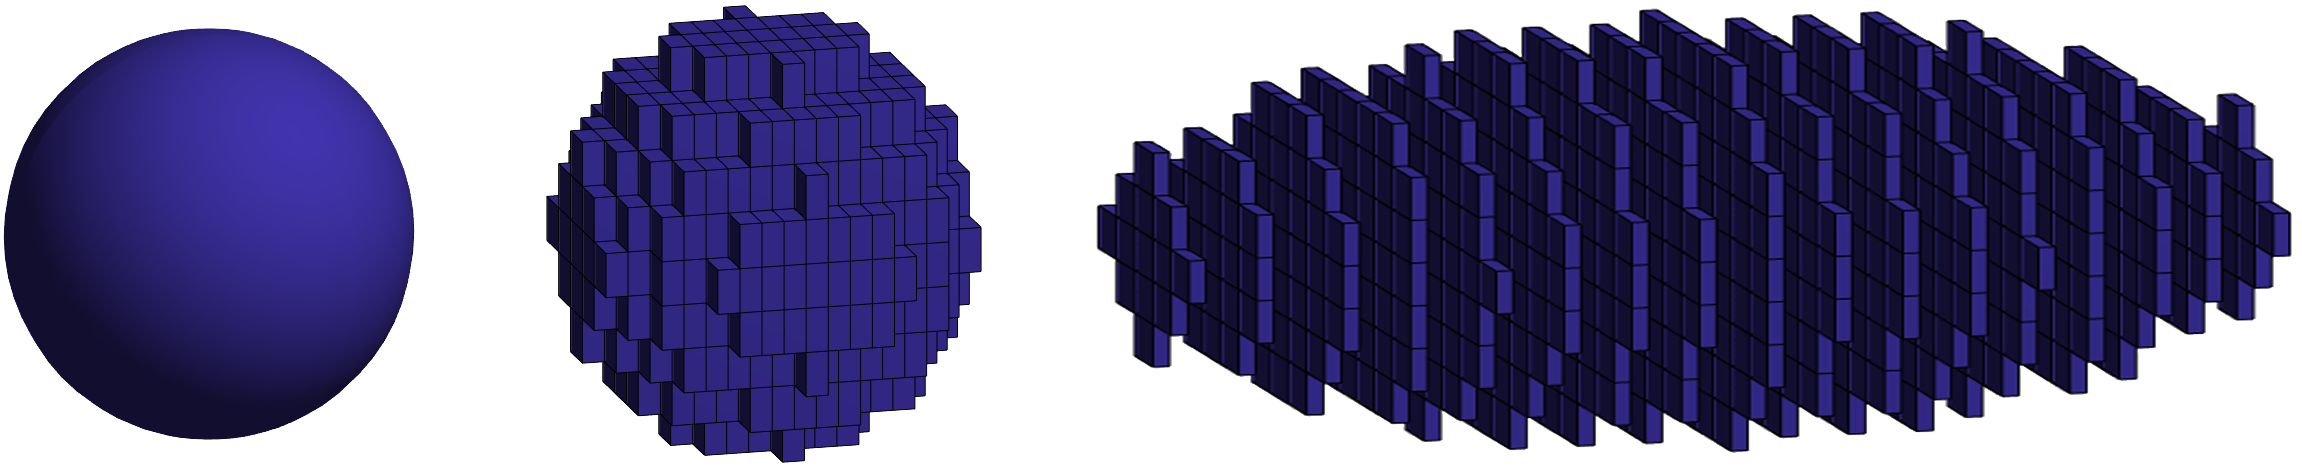
\includegraphics[width=1\textwidth]{images/multislice_sphere.png}
	\caption[Prinzip Multislice]{Prinzip der Multislice-Simulation: Das zu simulierende Streuobjekt (in diesem Fall eine einfache Kugel) wird in eine quaderförmige Szene eingebettet (wobei für die Berechnung eine größere x,y-Ausdehnung als z-Ausdehnung gewählt wird) und diskretisiert. Üblicherweise wird hierbei eine feinere Auflösung $\Delta z$ in Strahlrichtung gewählt. Bei der Simulation werden nun einzelne Schichten betrachtet.}
	\label{fig:multislice_prinzip}
\end{figure} 

Einer dieser Algorithmen ist die \textit{Multislice Fouriertransformation (MSFT)}. Nach \fref{eq:born} gilt in der ersten Bornschen Näherung für die Amplitude der gestreuten Welle
\begin{equation}
	\phi\propto\int \delta\eta(\vec{r}) e^{-i\vec{q}\cdot \vec{r}} \dif \vec{r} \, .
\end{equation}
Um die Komplexität zu reduzieren, wird nun versucht auf eine schichtweise Berechnung überzugehen: Wird das Skalarprodukt $\vec{q}\cdot \vec{r}=xq_x+yq_y+zq_z$ ausgeschrieben und die Integration über $x$ und $y$ als zweidimensionale Fouriertransformation interpretiert,
\begin{equation}
	\phi\propto\int \mathscr{F}\left[\delta\eta\right](q_x,q_y,z) e^{-izq_z} \dif z \, ,
\end{equation}

so lässt sich das Integral in z-Richtung als Summe interpretieren:
Aufgrund der Impulserhaltung muss für die Wellenvektoren $\vec{k_0}^2=\vec{k}^2=k^2$ gelten. Nach  \fref{fig:vec_msft} lässt sich der Streuvektor $\vec{q}$ in einen zum einfallenden Wellenvektor parallelen Anteil $\vec{q_\parallel}$ sowie einen senkrechten Anteil $\vec{q_\perp}$ zerlegen,
\begin{align}
	k^2=(k-q_\parallel)^2+q_{\perp}^2                  
	\Leftrightarrow q_\parallel=k-\sqrt{k^2-q_\perp^2} \,.
\end{align}
\begin{figure}
	\centering
	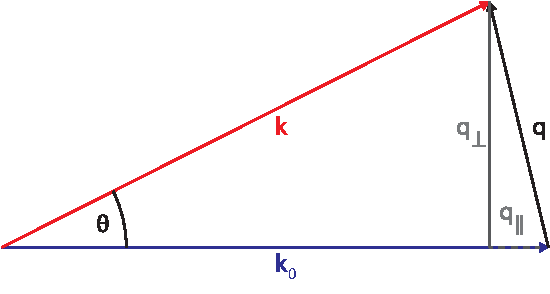
\includegraphics[width=0.5\textwidth]{images/vec_msft.pdf}
	\caption[Vektoren bei MSFT]{Skizze zur Bezeichnung der Vektoren. $\vec{k_{0}}$ und $\vec{k}$ bezeichnen den Wellenvektor der einfallenden bzw. ausfallenden Welle mit dem dazwischenliegenden Winkel $\theta$. $\vec{q}$ bezeichnet den Streuvektor mit einer zu $\vec{k_{0}}$ parallelen ($q_{||}$) und einer senkrechten ($q_\perp$) Komponente.}
	\label{fig:vec_msft}
\end{figure} 

Somit kann $q_z=q_\parallel$ eingesetzt werden und es gilt für die Welle im Fernfeld wie in \fref{fig:slice_msft} illustriert
\begin{equation}
	\label{eq:msft}
	\phi\approx\sum_n{\mathscr{F}\left[\delta\eta\right] e^{-in\delta_z\left(k-\sqrt{k^2-q_\perp^2}\right) }} \, .
\end{equation}

\fref{eq:msft} beschreibt einen Algorithmus um das Streubild eines dreidimensionalen Objektes im Fernfeld schichtweise in der ersten Bornschen Näherung zu berechnen~\cite{barke2015}. 

\begin{figure}
	\centering
	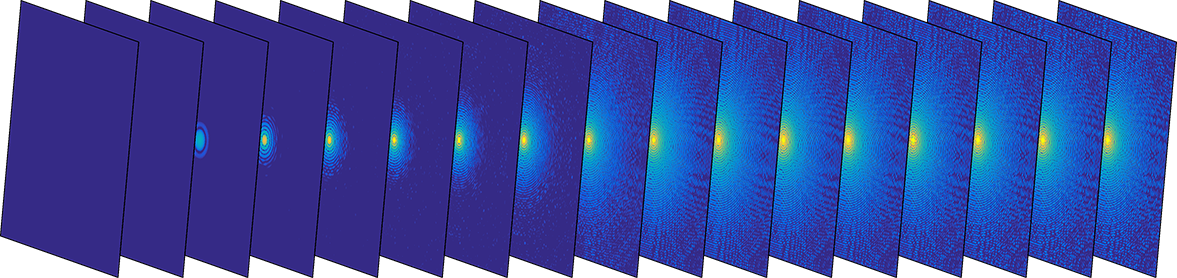
\includegraphics[width=1\textwidth]{images/slice_msft.pdf}
	\caption[Illustration MSFT]{Illustration zur MSFT: Das Streubild wird berechnet, indem schichtweise der jeweilige Beitrag der Bornschen Näherung phasenkorrekt aufaddiert wird. Die Position der dargestellten Schichten ist auf der z-Achse markiert. Das Bild unten rechts außen ist somit das berechnete Streubild des Objektes und das Ergebnis des Algorithmus.}
	\label{fig:slice_msft}
\end{figure} 

Bei dieser Methode wird Mehrfachstreuung vollständig ignoriert. Durch nachträgliches Einführen eines zusätzlichen Faktors, der die Absorption und Phasenänderung der Welle beim Durchlaufen des Objektes beschreibt, ließe sich nachträglich eine grobe Näherung für Absorptionseffekte einführen, die in einigen Fällen die subjektive Qualität der Simulation zu verbessern scheint~\cite{barke2015}. Da zum Einen die Gültigkeit dieser Absorptionsnäherung nicht direkt abgeschätzt werden kann und sie zum Anderen nicht in allen Fällen die Güte der Simulation verbessert, ist im Weiteren mit \textit{MSFT} die Methode ohne diese Korrektur bezeichnet~\cite{fennel}.
Eine Implementierung des MSFT-Algorithmus mit optionaler Absorptionskorrektur liegt in \texttt{simulation/msft.m} vor. 

\section{Multislice Propagation}
Ein alternatives Verfahren zur Simulation von Streubildern ist in der Literatur als \textit{Multislice Propagation} oder \textit{Beam Propagation} bekannt~\cite{hare1994,cowley1957}. Bei diesem in \fref{fig:multislice} skizzierten Verfahren wird zunächst die Szene ebenfalls in einzelne Schichten mit dem Abstand $\Delta z$ zerlegt. Jedoch unterscheidet sich das weitere Vorgehen deutlich von \textit{MSFT}: Statt auf der Born-Näherung zu basieren, wird schichtweise der Durchtritt der in die Szene einfallenden ebenen Welle durch das Objekt simuliert. Hierbei wird die Ausbreitung von Schicht zu Schicht genähert durch eine Vakuumpropagation nach \textit{Angular Spectrum Propagation} im Hybridraum\footnote{Die Näherung der Vakuumausbreitung durch einen Fresnel-Propagator bringt gegenüber der korrekten Berechnung über die Angular Spectrum Propagation keine numerischen Vorteile. Aus diesem Grund wird im Gegensatz zu~\cite{hare1994} auf diese Näherung verzichtet.},
\begin{equation}
	\bar{\phi}\left(q_x,q_y,z+\Delta z\right)=\bar{\phi}(z)e^{i\Delta z\sqrt{k^2-(q_x+q_y)^2}} \, ,
\end{equation}
sowie durch eine Wechselwirkung mit der Materie der Schicht in einer einzelnen Ebene im Realraum
\begin{equation}
	\phi(x,y,z+\Delta z)=\phi e^{i\delta n\left(z\right) \Delta z} \, .
\end{equation}
\begin{figure}
	\centering
	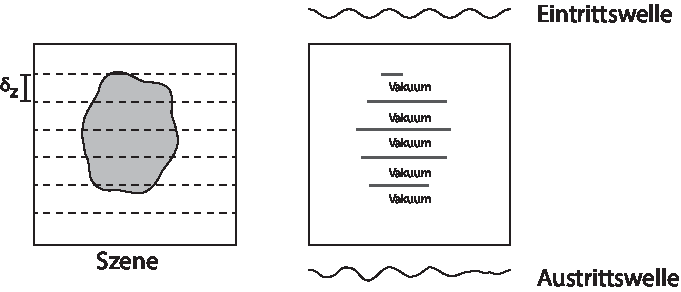
\includegraphics[width=0.9\textwidth]{images/multislice.pdf}
	\caption[Prinzip Multislice Propagation]{Prinzip der Multislice Propagation: Die Szene wird in einzelne Schichten zerlegt und die Wechselwirkung mit der Materie jeder einzelnen Schicht in auf eine in dieser Schicht liegenden Ebene reduziert. Zwischen diesen Ebenen wird eine Vakuumpropagation angewendet.}
	\label{fig:multislice}
\end{figure} 	

Dabei wird die Annahme getroffen, dass  innerhalb einer Schicht die örtliche Verteilung der Materie konstant ist, sowie die durch die Propagation bedingte Veränderung innerhalb von $\Delta z$ ausreichend klein ist, sodass keine Anteile der Wellenfront innerhalb einer Schicht unterschiedliche Brechzahlen durchlaufen~\cite{hare1994}. Dies kann durch ein hinreichend kleines $\Delta z$ gewährleistet werden. 
Des Weiteren wird bei der Wechselwirkung mit der Materie der Winkel mit dem ein Anteil der Wellenfront durch die Materie läuft vernachlässigt: Bei Anteilen der Welle, die durch vorangegangene Streueffekte bereits in einem deutlichen Winkel die Szene durchlaufen, wird genähert, dass ihr Weg durch die Materie gleich lang wie der Weg von nicht gestreuten Anteilen ist. Somit wird Mehrfachstreuung zwar mitberücksichtigt, jedoch nur näherungsweise.
	
Der Algorithmus zur Berechnung der Austrittswelle, d.h. der Welle hinter der Szene bzw. dem Streuobjekt, ist somit die iterative Anwendung von
\begin{equation}
	\label{eq:multislice}
	\Phi(z+\Delta z)= e^{i\delta n\left(z\right) \Delta z}\mathscr{F}^{-1}\left[e^{i\Delta z\sqrt{k^2-(q_x+q_y)^2}}\mathscr{F}\left[\Phi(z)\right]\right] \,.
\end{equation}
Dies ist in \fref{fig:slice_multislice} am Beispiel der Austrittswelle hinter einer Kugel illustriert.

Ist die Austrittswelle bekannt, so ist die weitere Ausbreitung zum Detektor eine Vakuumpropagation, die sich entweder mittels \textit{Angular Spectrum Propagation} berechnen, oder durch eine einfache Fouriertransformation in Fraunhofer-Näherung bestimmen lässt. Ersteres Verfahren hat den Nachteil, das es bei einer numerischen Implementierung im Bereich der Szene die gleiche räumliche Rastergröße wie im Bereich des Detektors erfordert. Bei Anwendung der Fernfeldnäherung ist zwar der maximale Winkel, in dem das Streubild berechnet werden kann, von der räumlichen Auflösung der Austrittswelle sowie die Winkelauflösung von der Szenenausdehnung abhängig, dies ist jedoch deutlich praktikabler.
Diese Methode wird im Weiteren als \textit{Multislice Propagation} bezeichnet und ist in \texttt{simulation/multislice.m} implementiert.

\begin{figure}
	\centering
	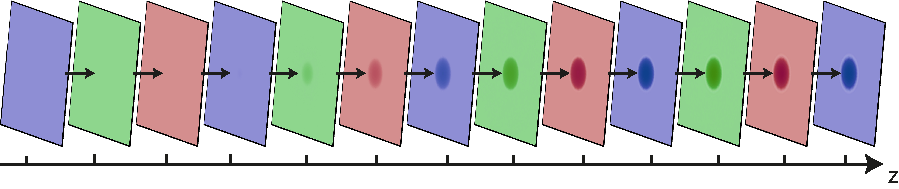
\includegraphics[width=1\textwidth]{images/slice_multislice.pdf}
	\caption[Illustration Multislice Propagation]{Illustration zur Multislice Propagation: Bei Strahlrichtung von links nach rechts ist von exemplarischen (auf der z-Achse markierten) Schichten  der Betrag der komplexen Wellenfront als Helligkeit, die Phase als Farbton dargestellt. Rechts außen ist die Austrittswelle hinter der Szene und damit das Ergebnis des Algorithmus.}
	\label{fig:slice_multislice}
\end{figure} 
	
\section{Thibaults Multislice}
Thibault hat in~\cite{thibault2007} eine eigene Formulierung der Multislice-Simulation aufgestellt. Ausgehend von der Wellengleichung (\fref{eq:wellengleichung_green})
lässt sich für die Welle im Hybridraum 
\begin{equation}
	\bar{\Phi}(z)=\bar{G}\ast_z\left[\bar{\delta\eta}\ast_{q_\perp} \bar{\Phi}\right]
\end{equation}
mit
\begin{equation}
	\bar{G}=\frac{1}{2\pi}\frac{ik^2}{\sqrt{k^2-q_\perp^2}}e^{iz(q_\parallel-k)}
\end{equation}
aufstellen. Hierbei sind die Faltungsoperatoren mit den Variablen, über die die Faltung durchzuführen ist, indiziert.
Wird nun die Welle bei $\Delta z$ betrachtet, so lässt sich unter Vernachlässigung von Rückstreuung  das Faltungsintegral über $z$ in zwei Integrationsbereiche aufspalten (vom Ursprung bis $\Delta z$ sowie von dort bis ins Unendliche):
\begin{equation}
	\bar{\Phi}(z+\Delta z)=
	\int_{\Delta z}^{\infty} \bar{G}(z')\left[\bar{\delta\eta}\ast_{q_\perp} \bar{\Phi}\right](z+\Delta z-z')\dif z'
	+
	\int_{0}^{\Delta z} \bar{G}(z')\left[\bar{\delta\eta}\ast_{q_\perp} \bar{\Phi}\right](z+\Delta z-z')\dif z' \,.
\end{equation}
Für den ersten Summanden gilt mit einer Substitution ($z'\rightarrow z''+\Delta z$)
\begin{align*}
	  & \stackrel{\hphantom{z'\rightarrow z''+\Delta z}}{\hphantom{=}} 
	\int_{\Delta z}^{\infty} \bar{G}(z')\left[\bar{\delta\eta}\ast_{q_\perp} \bar{\Phi}\right](z+\Delta z-z')\dif z'\\
	  & \stackrel{z'\rightarrow z''+\Delta z}{=}                       
	\int_{0}^{\infty} \bar{G}(z''+\Delta z)\left[\bar{\delta\eta}\ast_{q_\perp} \bar{\Phi}\right](z-z'')\dif z''\\
	  & \stackrel{\hphantom{z'\rightarrow z''+\Delta z}}{=}            
	e^{i\Delta z(q_\parallel-k)}\int_{0}^{\infty} \frac{1}{2\pi}\frac{ik^2}{\sqrt{k^2-q^2_\perp}}e^{iz''(q_\parallel-k)}\left[\bar{\delta\eta}\ast_{q_\perp} \bar{\Phi}\right](z-z'')\dif z''\\
	  & \stackrel{\hphantom{z'\rightarrow z''+\Delta z}}{=}            
	e^{i\Delta z(q_\parallel-k)}\bar{\Phi}(z) \numberthis \,,
\end{align*}
im zweiten Summanden kann für hinreichend kleine $\Delta z$ das Integral gut durch eine Rieman-Obersumme mit einem einzigen Stützpunkt bei $\Delta z$ approximiert werden (der Fehler ist hierbei von der Ordnung $\Delta z$):
\begin{equation}
	\int_{0}^{\Delta z} \bar{G}(z')\left[\bar{\delta\eta}\ast_{q_\perp} \bar{\Phi}\right](z+\Delta z-z')\dif z'
	\approx
	\Delta z \bar{G}(\Delta z)\left[\bar{\delta\eta}\ast_{q_\perp} \bar{\Phi}\right](z) \,.
\end{equation}
Somit lässt sich in Näherung für die Welle bei $z+\Delta z$
\begin{equation}
	\label{eq:thibault}
	\bar{\Phi}(z+\Delta z)
	\approx
	e^{i\Delta z(q_\parallel-k)}
	\left(
	\bar{\Phi}(z)+\frac{\Delta z}{2\pi}\frac{ik^2}{\sqrt{k^2-q^2_\perp}}  \left[\bar{\delta\eta}\ast_{q_\perp} \bar{\Phi}\right](z)
	\right)
\end{equation}
aufstellen. Dies stellt eine iterative Beschreibung der Streuung dar -- ausgehend von $z=0$ kann schrittweise in Einfallsrichtung die Wellengleichung in einer Szene gelöst werden. Somit handelt es sich um einen Algorithmus, der ebenfalls der Kategorie "`Multislice"' zuzuordnen ist. Im Gegensatz zur \textit{Multislice Propagation} findet hier die Wechselwirkung mit der Materie jedoch nicht in Form eines Exponentialfaktors statt, in Kleinwinkelnäherung entspricht \fref{eq:thibault} einer Taylornäherung erster Ordnung in der Exponentialfunktion von \fref{eq:multislice}. Unabhängig von der Gültigkeit der verwendeten Näherungen besitzt \fref{eq:thibault} bei $k^2=q_\perp$ eine Singularität. Aus diesem Grund muss entweder das Raster, in dem die Simulation durchgeführt wird, hinsichtlich der Auflösung in x,y-Richtung so gewählt werden, dass diese Singularität nicht zum Tragen kommt oder nach jedem Simulationsschritt im Fourierraum $\bar{\Phi}(q_x,q_y)$ für $q_x+q_y>k$ auf Null gesetzt werden.
Die numerische Simulation dieser Methode ist in \texttt{simulation/thibault.m} implementiert.


\section{Verifizierung}
Zur Verifizierung der vorgestellten Simulationsalgorithmen und deren numerische Implementierungen eignet sich der Vergleich der berechneten Streubilder hinter Kugeln mit den Ergebnissen aus der Berechnung mittels Mie-Streuung. Der Vergleich wird für verschiedene Brechzahlen und Kugelradien bei einer Wellenlänge von \SI{1}{nm} durchgeführt.

Da ein realer Detektor nicht die Intensitäten bei präzise definierten Winkelpunkten misst, sondern innerhalb eines Areals, ist es zweckmäßig, die simulierte Detektorfläche in quadratische Areale (\textit{Pixel}) zu unterteilen und die Intensität in jedem dieser Areale als gewichtetes Mittel zwischen in dem Areal liegenden Punkten zu betrachten.
Hierbei werden (wie in \fref{fig:average} dargestellt) an den Rändern zwischen zwei Arealen liegende Berechnungspunkte je zur Hälfte in beiden Arealen, in der Ecke zwischen vier Arealen liegende Berechnungspunkte je zu einem Viertel in den vier Arealen berücksichtigt.
Besonders bemerkbar ist dieser Bearbeitungsschritt bei Pixeln die genau in den Intensitätsminima liegen: Ohne die gewichtete Mittlung würde der gesamten Fläche zwischen den Pixeln die Intensität des Minimums zugewiesen werden, auch wenn dessen Breite extrem schmal ist, werden zusätzliche Pixel berechnet und anschließend gewichtet gemittelt, ergibt sich eine korrektere Wiedergabe des tatsächlichen Intensitätsverlaufs. Dies wird sowohl für die mit den verschiedenen Algorithmen simulierten Streubildern als auch für die Mie-Streubilder durchgeführt und einspricht einer einfachen Form des \textit{Antialiasings}, das den Einfluss der diskreten Berechnung verringert.
\begin{figure}[b] %mittelwert
	\centering
	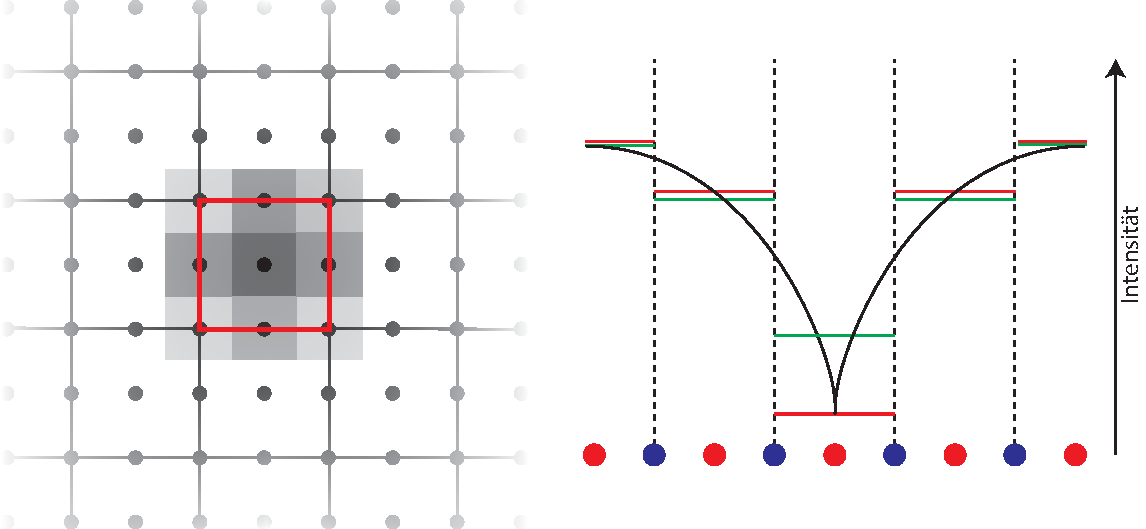
\includegraphics[width=0.9\textwidth]{images/average.pdf}
	\caption[Gewichteter Mittelwert]{Die Verwendung von Überabtastung und gewichteten Mittelwertes bei den Streubildern: Um die Intensität im links rot umrandeten Bereich zu bestimmen, wird die Intensität an den schwarzen Punkten berechnet und ein gewichteter Mittelwert gebildet. Dazu wird die Intensität der vier Randwerte zur Hälfte, die der vier Eckpixel zu einem Viertel in dem umrandeten Bereich mitberücksichtigt. Der Effekt gegenüber einer simplen Berechnung des zentralen Pixels zeigt sich rechts: Wird die Intensität bei einem schwarz dargestellten wahren Intensitätsverlauf nur an den roten Punkten bestimmt, dominiert das Minimum den Intensitätsverlauf. Eine geringere Abweichung ergibt sich bei Berechnung auch an den blauen Punkten und anschließender Bildung des gewichteten Mittelwerts (grün).}
	\label{fig:average}
\end{figure}% 

Anschließend werden die simulierten Streubilder bezüglich ihrer Skalierung auf die Mie-Streubilder normiert. Hierzu wird ein Skalierungsfaktor gesucht, der die mittlere Abweichung der simulierten Streubilder vom jeweiligen Mie-Streu"-bild innerhalb der ersten 10° minimiert. Zur Quantifizierung des Fehlers der simulierten Streubilder wird die relative Abweichung von den Mie-Streu"-bildern betrachtet. Für die \textit{Multislice Propagation} ist in \fref{fig:exitscatter} für einen konkreten Parametersatz exemplarisch Austrittswelle und Streubild dargestellt, die relative Abweichung von Mie ist für diesen Parametersatz in \fref{fig:relerror} für alle Simulationsansätze dargestellt. 

\begin{figure} %exitwave und scatter
	\centering
	\begin{subfigure}[b]{0.4\textwidth}
		\setbox1=\hbox{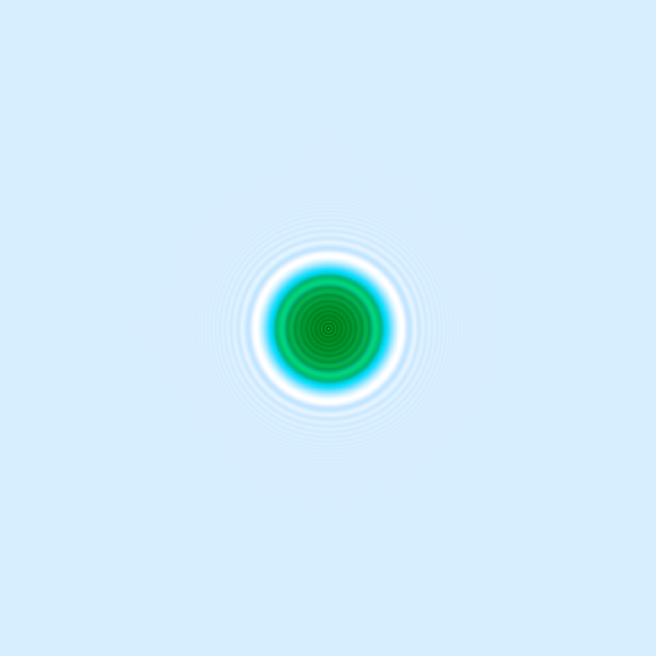
\includegraphics[width=\textwidth]{images/fig_sim_exitwave_multislice-r100-bd1e-3.png}}
		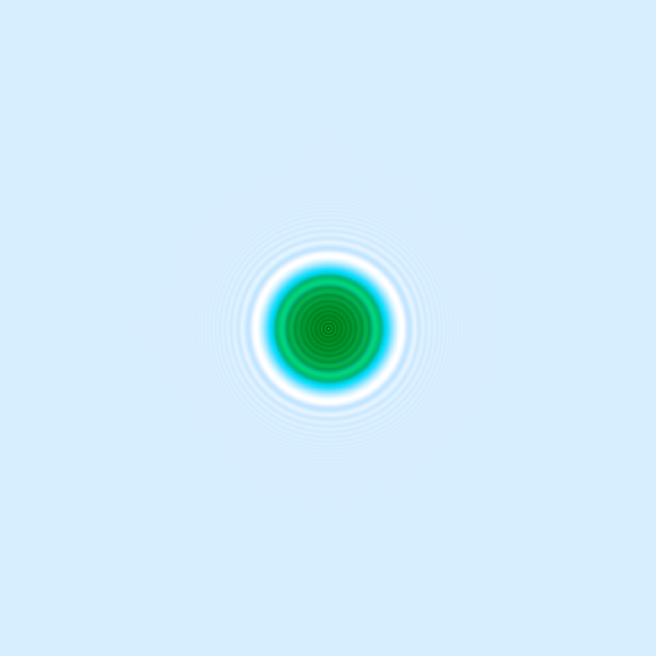
\includegraphics[width=\textwidth]{images/fig_sim_exitwave_multislice-r100-bd1e-3.png}\llap{\makebox[\wd1][l]{\includegraphics[width=0.4\textwidth]{images/fig_sim_exitwave_multislice_cw-r100-bd1e-3.pdf}}}
		\caption{Austrittswelle}
		\label{fig:exitwave}
	\end{subfigure}
	\hspace{1.5cm}
	\begin{subfigure}[b]{0.4\textwidth}
		\setbox1=\hbox{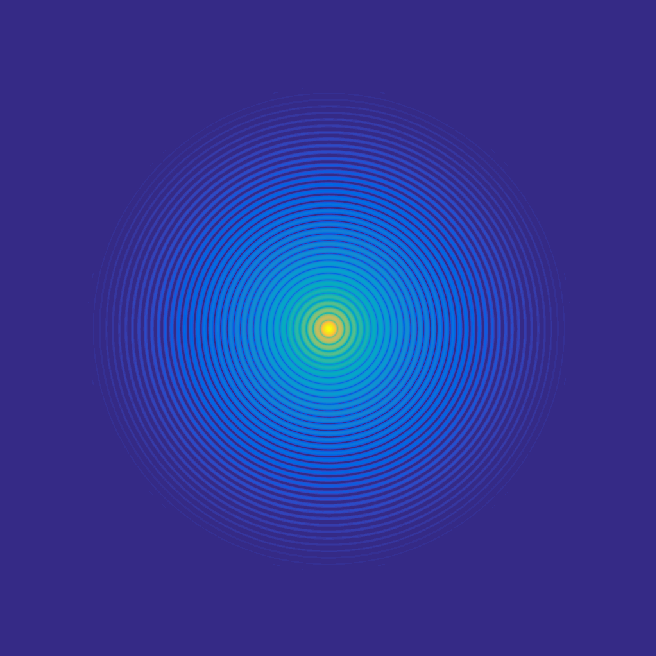
\includegraphics[width=\textwidth]{images/fig_sim_scatter_multislice-r100-bd1e-3.png}}
		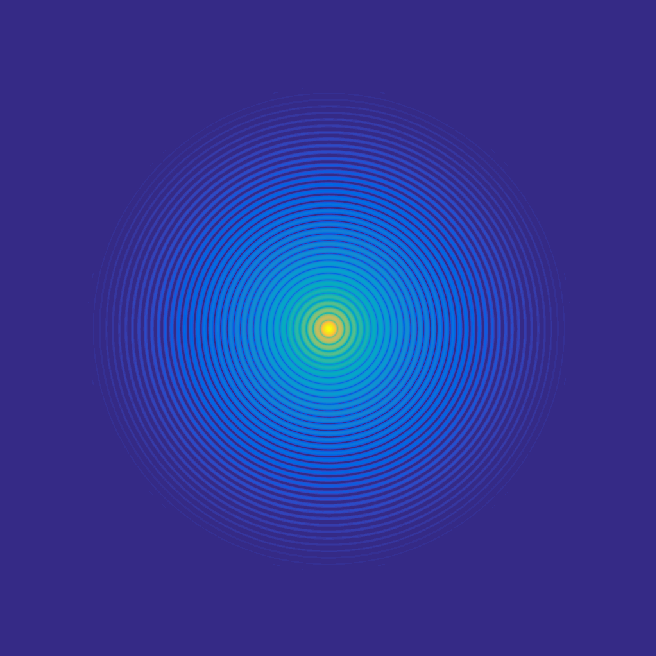
\includegraphics[width=\textwidth]{images/fig_sim_scatter_multislice-r100-bd1e-3.png}\llap{\makebox[\wd1][l]{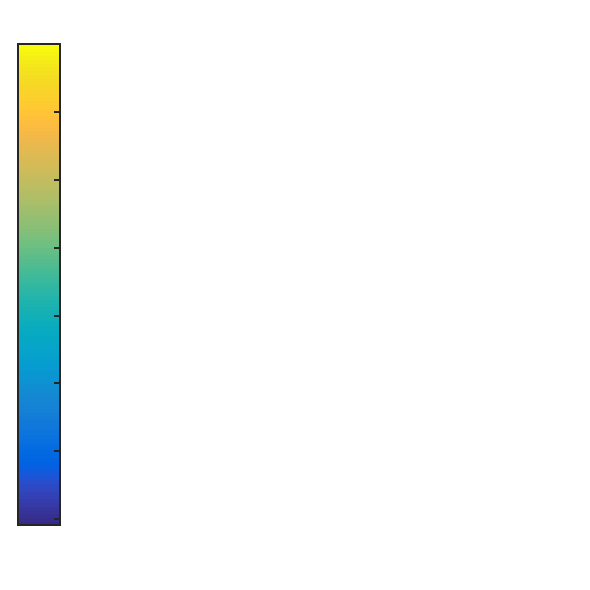
\includegraphics[width=0.5\textwidth]{images/fig_sim_scatter_multislice_cb-r100-bd1e-3.pdf}}}
		\caption{Streubild}
		\label{fig:scatter}
	\end{subfigure}
	\caption[Austrittswelle und Streubild einer Kugel]{Exemplarische Multislice-Propagations Austrittwelle (a) und logarithmierte Intensität des simulierten Streubildes (b) einer Kugel mit Radius \SI{100}{nm} bei $\beta,\delta$=$10^{-3}$. Die relative Intensität der Austrittswelle bezüglich der Eintrittswelle ist über die Helligkeit dargestellt, die Phase über den Farbton. Das Streubild zeigt einen Bereich bis 15°.}
	\label{fig:exitscatter}
\end{figure}%

Aus den rotationssymmetrischen Streubildern können nun Radialprofile der Intensität sowie des relativen Fehlers bestimmt werden um einen besseren Überblick zu erhalten (\fref{fig:profil}). Es ist zu erkennen, dass der relative Fehler in den Datenpunkten, in denen das Mie-Profil ein Minimum hat, aufgrund dessen steilen Verlaufs scharfe, nur 1-2 Datenpunkte umfassende, Maxima annimmt. Um die Güte einer Simulation bei einem bestimmten Radius und Stoffeigenschaften zu quantifizieren, wird deshalb der Median des relativen Fehlers bis 20° Streuwinkel genutzt. So ist es möglich, für die unterschiedlichen Simulationsalgorithmen Bereiche zu bestimmen, in denen sie ausreichend mit der Mie-Theorie übereinstimmen, um sie dort als valide anzusehen. In \fref{fig:variation} wird deutlich, dass bei Werten von $\delta$ bzw. $\beta$ in der Größenordnung bis $10^{-4}$ (die viele Materialien bei \SI{1}{nm} Wellenlänge aufweisen~\cite{henke}) sowohl \textit{Multislice Propagation} und \textit{Thibaults Multislice} als auch \textit{MSFT} valide Ergebnisse liefern -- der mediane Fehler überschreitet 5~\% nicht. Bei größeren Abweichungen der Brechzahl von der Vakuumbrechzahl steigt der mediane Fehler des mittels \textit{MSFT} berechneten Streubildes deutlich an, insbesondere bei großen Radien. Bei diesen kommt es zu deutlich mehr Absorption und Mehrfachstreuung in Vorwärtsrichtung, die bei \textit{MSFT} im Gegensatz zu den beiden anderen Multislice Varianten vollständig ignoriert wird. Der Unterschied zwischen Thibaults Formulierung und der \textit{Multislice Propagation} kann zu einem gewissen Anteil durch die hier verwendete numerische Implementierung von Thibaults Algorithmus begründet sein. Hier besteht weiteres Optimierungspotential bezüglich der Genauigkeit und dem Einfluss von Rundungsfehlern.

\begin{figure} %rel error
	\centering
	\begin{subfigure}[b]{0.48\textwidth}
		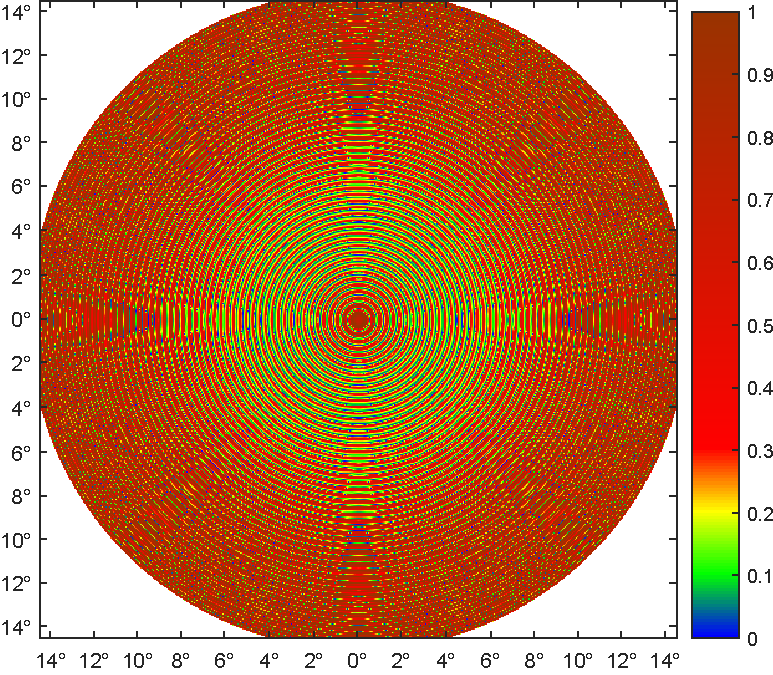
\includegraphics[width=\textwidth]{images/fig_sim_relerror_FTproj-r100-bd1e-3.pdf}
		\subcaption{Projektion}
	\end{subfigure}\hfill
	\begin{subfigure}[b]{0.48\textwidth}
		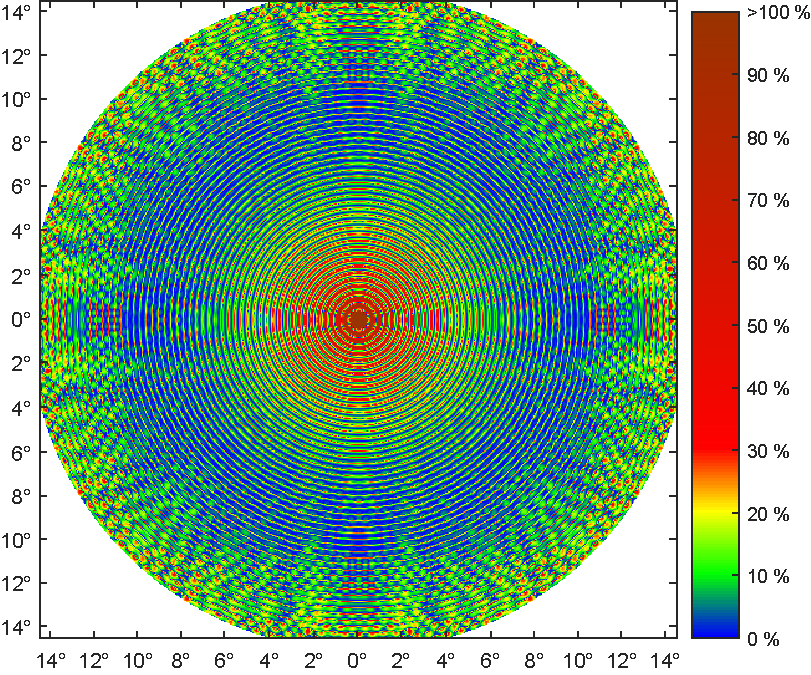
\includegraphics[width=\textwidth]{images/fig_sim_relerror_msft-r100-bd1e-3.pdf}
		\subcaption{MSFT}
	\end{subfigure}
	\par \vspace{1.5\bigskipamount}
	\begin{subfigure}[b]{0.48\textwidth}
		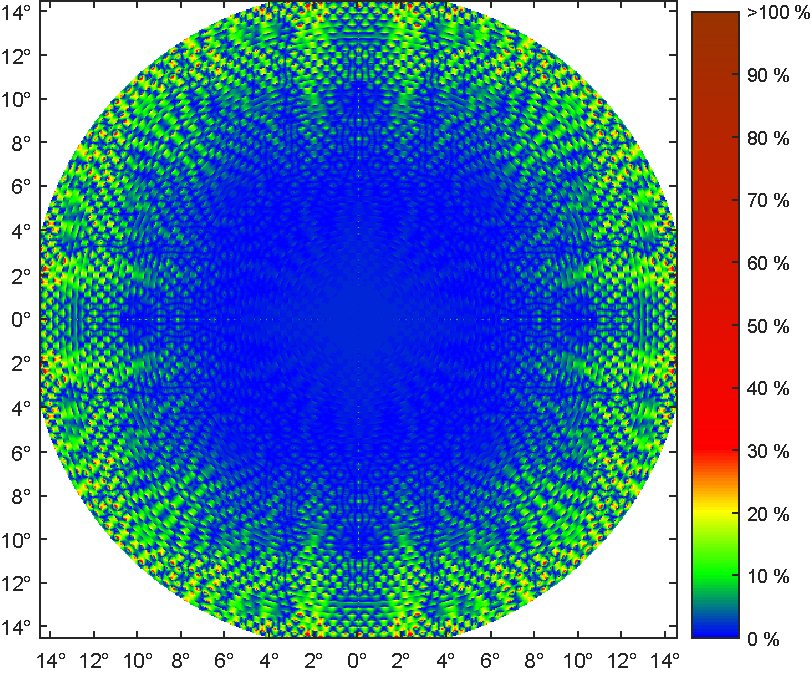
\includegraphics[width=\textwidth]{images/fig_sim_relerror_thibault-r100-bd1e-3.pdf}
		\subcaption{Thibaults Multislice}
	\end{subfigure}\hfill
	\begin{subfigure}[b]{0.48\textwidth}
		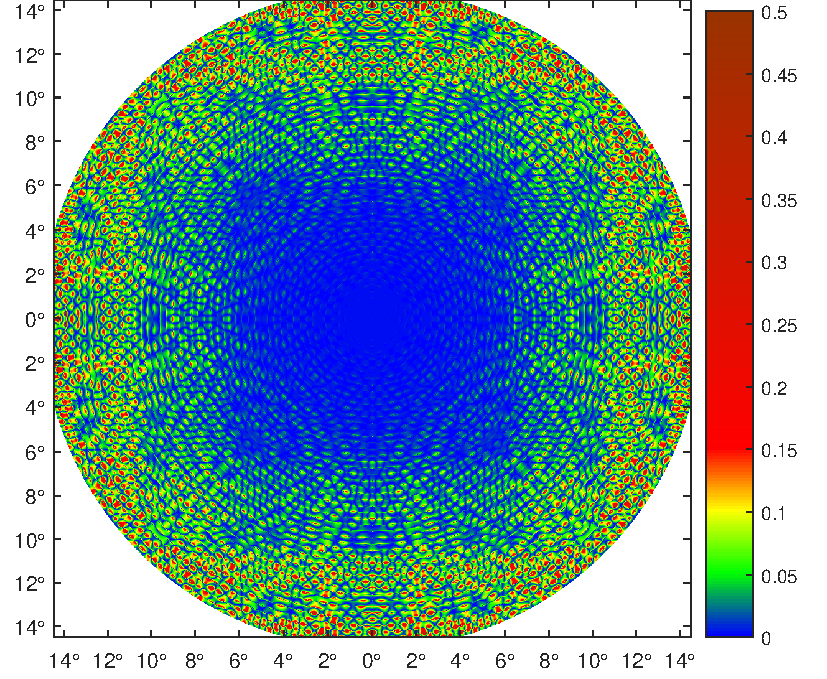
\includegraphics[width=\textwidth]{images/fig_sim_relerror_multislice-r100-bd1e-3.pdf}
		\subcaption{Multislice Propagation}
	\end{subfigure}
	\caption[Relativer Fehler der Simulationen]{Betrag der relativen Abweichungen von Mie der simulierten Streubilder einer Kugel mit Radius \SI{100}{nm} bei $\beta=\delta=10^{-3}$. Es ist bei allen Simulationsmethoden der Trend zu ansteigenden Abweichung bei größeren Streuwinkeln sowie konzentrische Zonen höherer Abweichungen zu erkennen. Bei den hier verwendeten Parametern zeigt die Projektionsnäherung ein deutlich schlechteres Ergebnis als die Multislice Ansätze.}
	\label{fig:relerror}
\end{figure}

\clearpage
\begin{sidewaysfigure} %profile
	\centering
	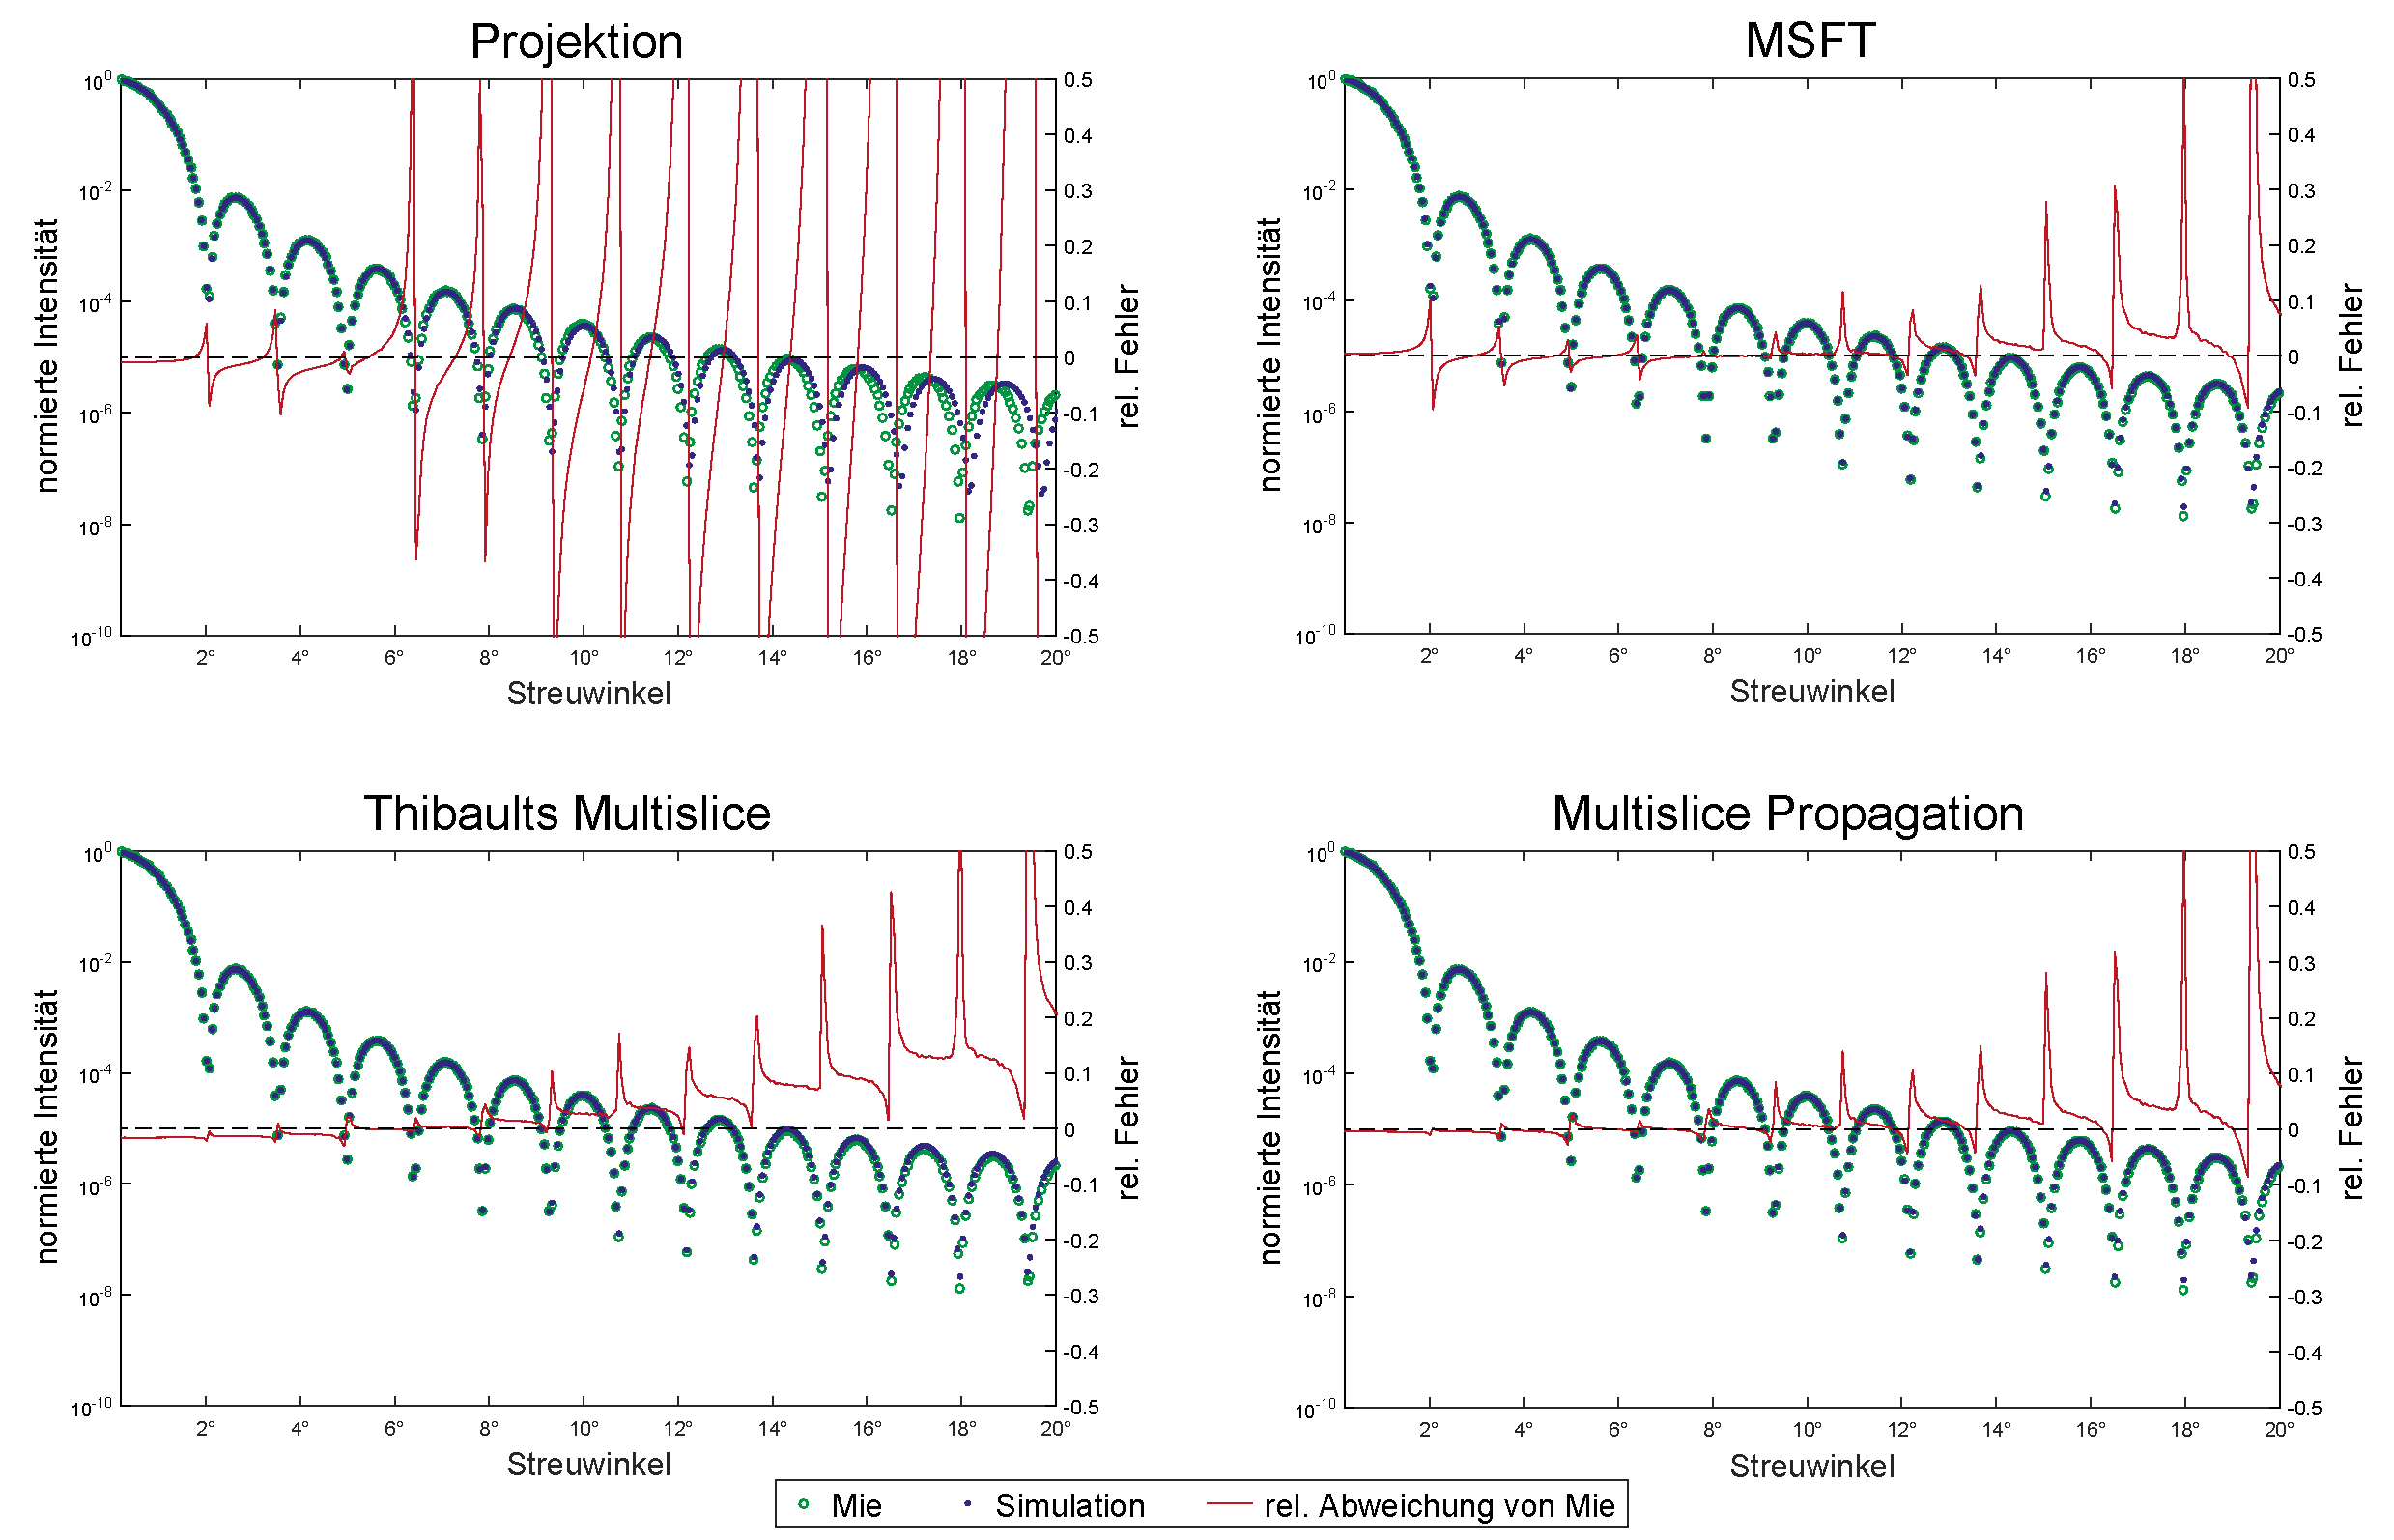
\includegraphics[width=1\textwidth]{images/fig_sim_profile.pdf}
	\captionsetup{width=0.95\textwidth}
	\caption[Radiale Profile]{Radiale logarithmierte Intensitätsprofile berechnet mit den verschiedenen Algorithmen sowie die relative Abweichung von Mie für eine Kugel mit Radius \SI{20}{nm} und $\beta,\delta$=$10^{-4}$. Es ist bei kleinen Streuwinkeln eine gute Übereinstimmung aller Algorithmen zu erkennen, bei größeren Winkeln versagt die Projektion. Über den gesamten Bereich besitzt bei diesen Parametern die Multislice Propagation die beste Übereinstimmung. Die relativen Fehler der Simulationen sind in den Intensitätsminima aufgrund der dort deutlich abfallenden Referenzintensität bei allen Verfahren stärker ausgeprägt.}
	\label{fig:profil}
\end{sidewaysfigure}
\clearpage

\begin{figure} %parameter variation
	\centering
	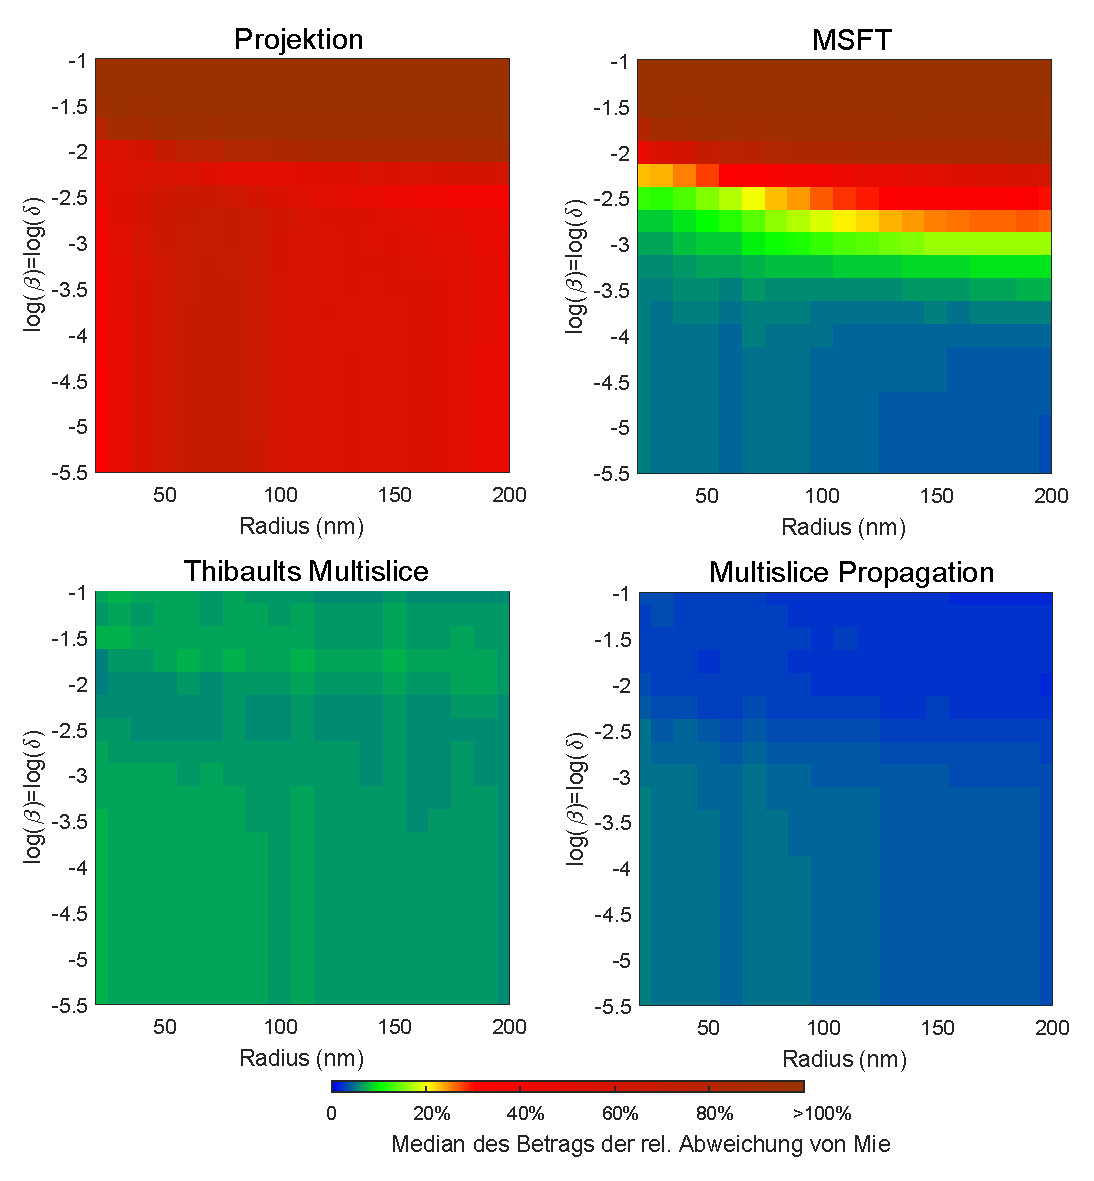
\includegraphics[width=1\textwidth]{images/fig_sim_var.pdf}
	\caption[Gültigkeit der Simulationsalgorithmen]{Zur Entscheidung bei welchen Radien und welchen Abweichungen der Brechzahl vom Vakuum die Simulationen noch valide sind, ist der Median des Betrags der relative Abweichung bis 20° von Mie über den Parametern aufgetragen. Es sind somit die Bereiche erkennbar, in denen der jeweilige Simulationsalgorithmus valide Ergebnisse liefert. Es ist insbesondere zu erkennen, dass bei größeren Brechzahlen sowie größeren Abweichungen von der Vakuumbrechzahl \textit{MSFT} nur eingeschränkt valide ist, sowie dass die \textit{Multislice Propagation} und \textit{Thibaults Multislice} über den gesammten dargestellten Bereich gute Ergebnisse liefern. Parameter: $\Delta x=\sfrac{\lambda}{2}$, $\Delta z$ und $\sfrac{\lambda}{8}$ und N=2048.}
	\label{fig:variation}
\end{figure}

Mit der \textit{Multislice Propagation} ist somit ein effizienter, schichtweise arbeitender Algorithmus gefunden, der sich für die Simulation synthetischer Streubilder eignet.


\section{Streubilder komplexer Objekte}
Neben der bislang zur Validierung erfolgten Berechnung von Streubildern von Kugeln eignen sich die Simulationsalgorithmen auch zur Berechnung der Austrittswellen und Streubilder hinter anderen, komplexeren Objekten. 

Als interessante Testszene wird das in \fref{fig:komplexmodel} dargestellte Modell einer wassergefüllte ikosaederförmige Lecithin-Membran (Außenradius \SI{375}{nm}, Dicke \SI{25}{nm}), um deren Mittelpunkt vier kleinere, DNA gefüllte Kugeln (Radius \SI{90}{nm}) in den Eckpunkten eines Tetraeders angeordnet sind, als biologisches Objekt betrachtet. Als Referenz dient ein disjunktes Xenon-Dodekaeder mit Außenradius \SI{100}{nm}. Die komplexen Brechzahlen der simulierten Materialien sind in \fref{tab:brechzahl} aufgeführt~\cite{henke,bergh2008,milo2015}. Die für diese Szene berechnete komplexe Austrittswelle ist in \fref{fig:komplexexit} gezeigt. Es sind sowohl die Wirkung der Absorption in Form der Intensitätsabnahme hinter den Streuobjekten, wie auch der Brechung in Form einer geringen Intensitätszunahme um die Streuobjekte sowie einer Phasenänderung zu erkennen. Das zugehörige Streubild ist in \fref{fig:komplexscatter} gezeigt und stellt das Ergebnis der Bemühungen synthetische Streubilder zu erstellen dar. Im Folgenden wird dies für den Vergleich der Rekonstruktionsansätze genutzt, indem deren Eignung zur Rekonstruktion der Austrittswelle betrachtet wird.


\begin{figure}[b]
	\centering
	\begin{minipage}[t]{.39\textwidth}
		\centering
		\vspace{0pt}
		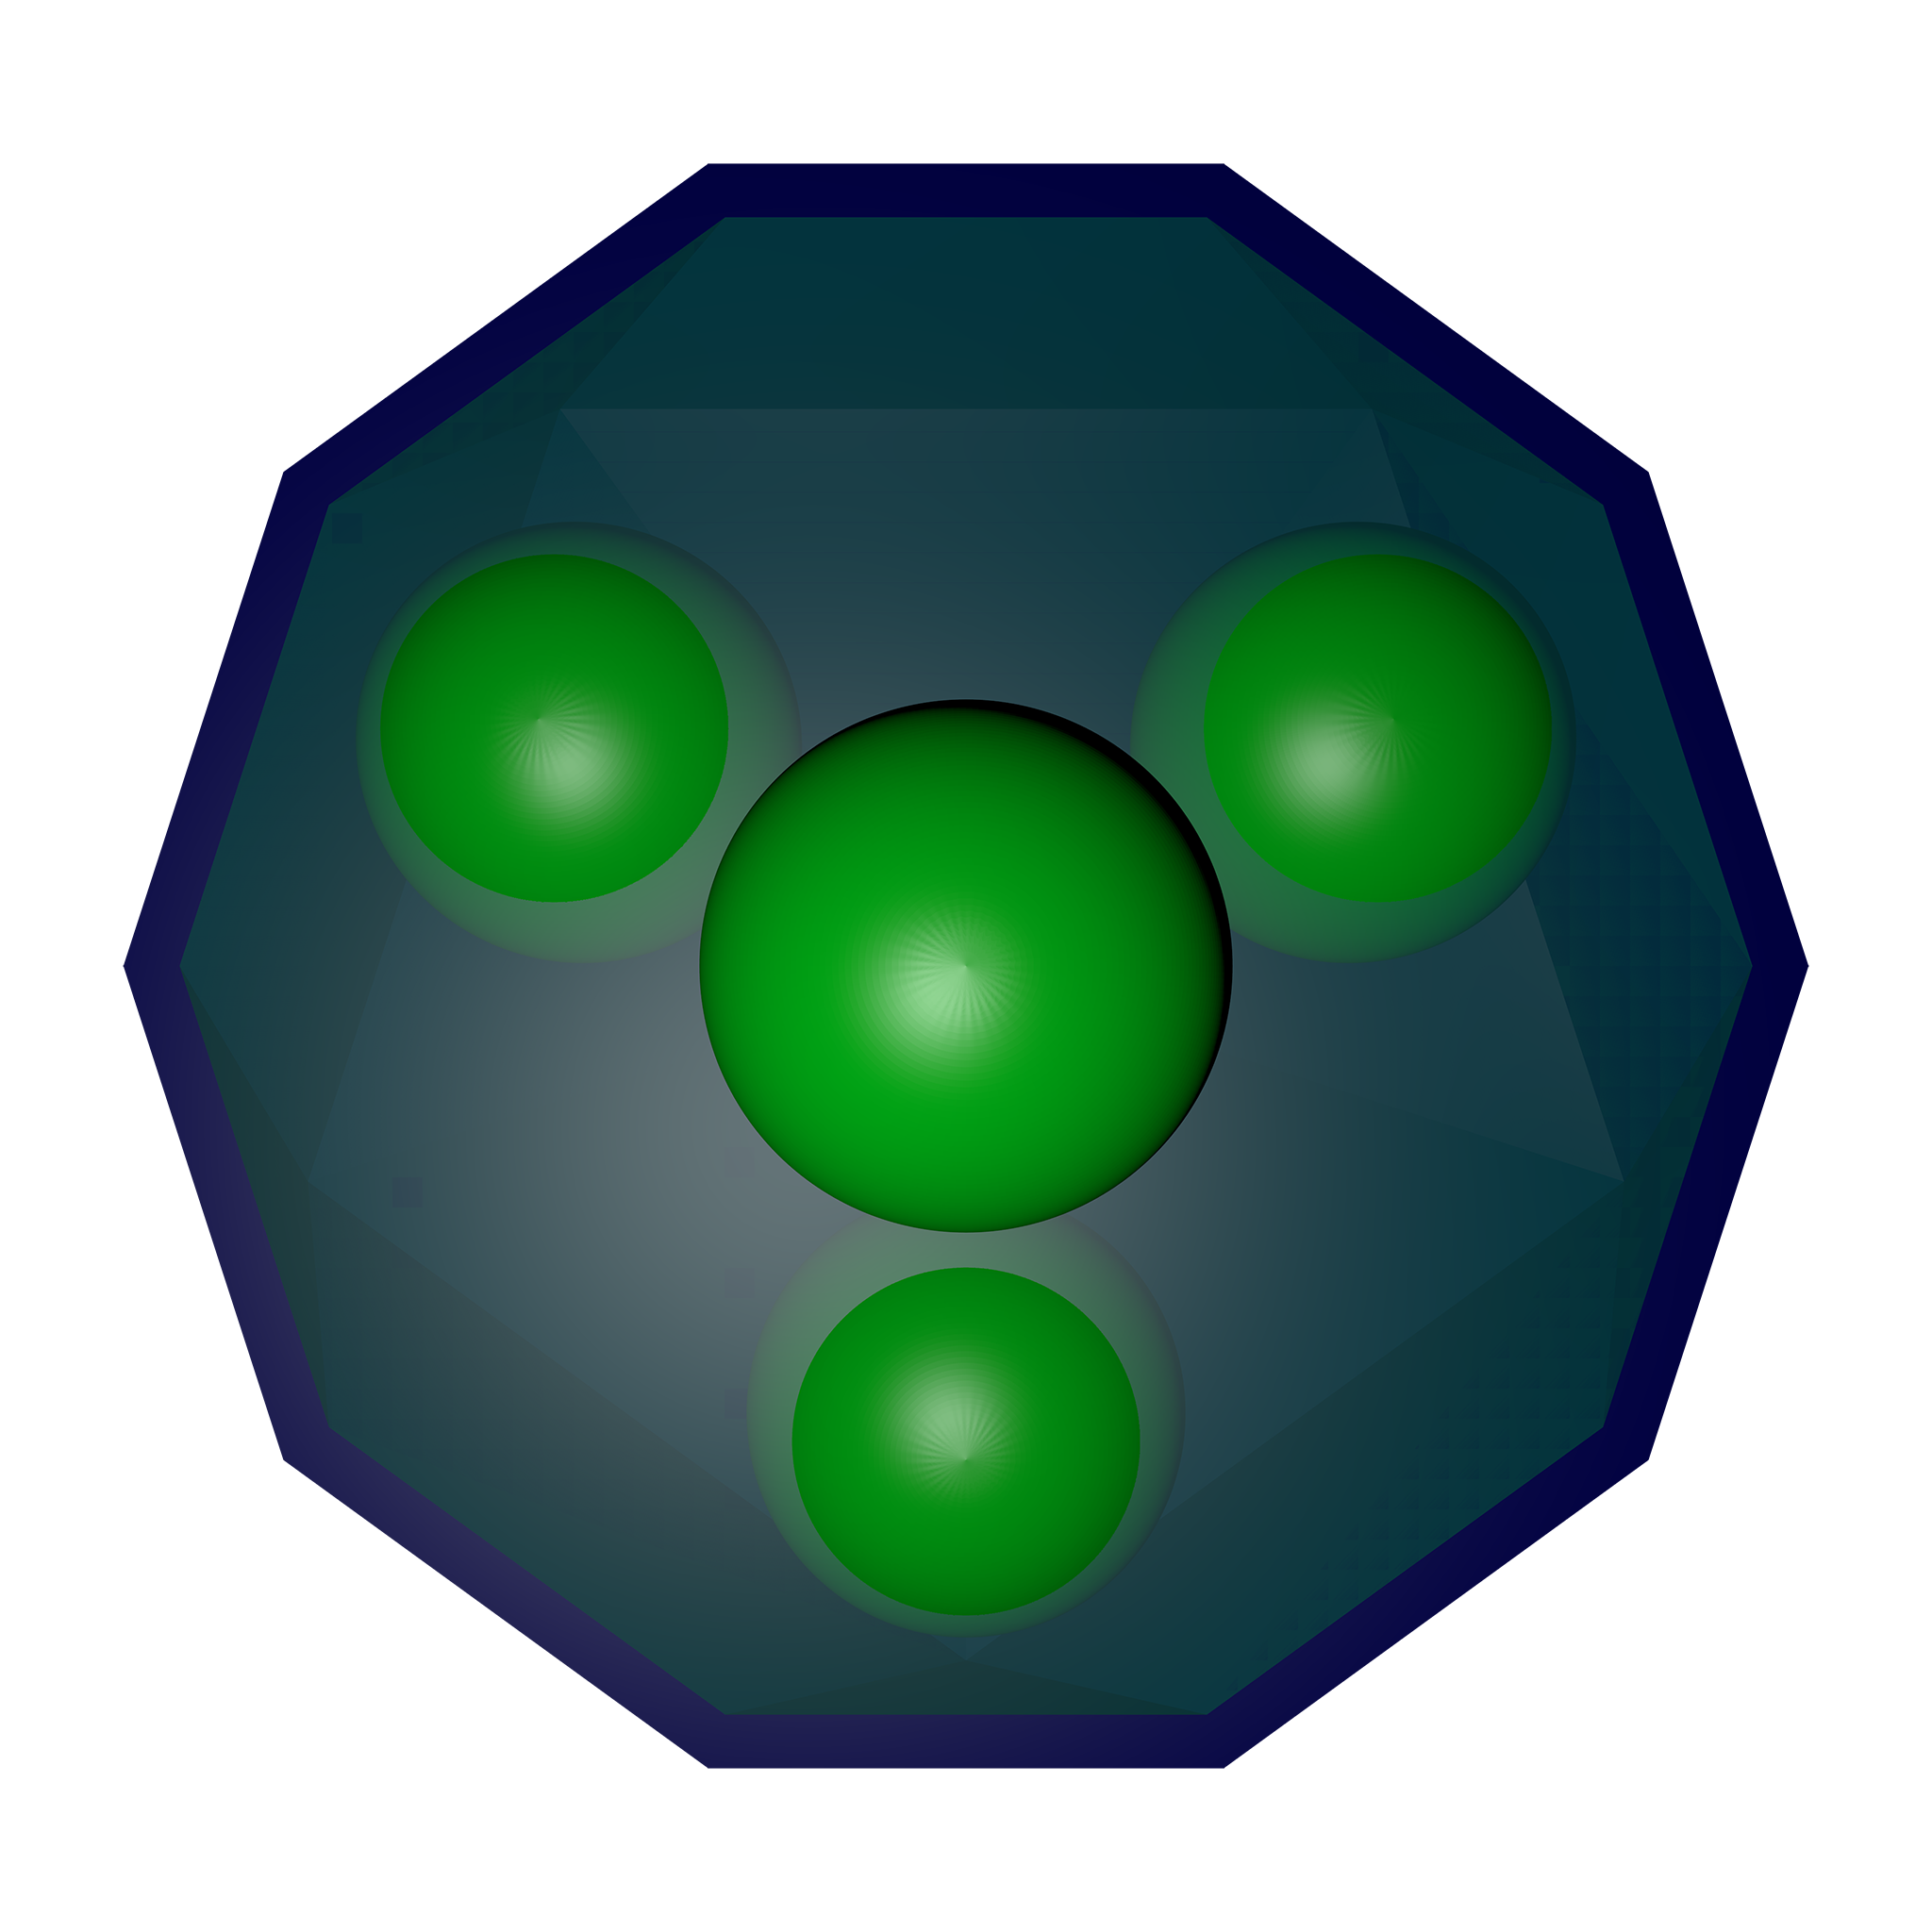
\includegraphics[width=0.7\textwidth]{images/scene.png}
		\caption{3D-Modell des Objektes\label{fig:komplexmodel}}
	\end{minipage}\hfill
	\begin{minipage}[t]{.60\textwidth}
		\centering
		\vspace{0pt}
		\captionof{table}{Für die Berechnung der komplexen Austrittswelle\\ verwendete Materialien \label{tab:brechzahl} }
			\begin{tabular}{lll}
				\hline
				Material													&Brechzahl bei \SI{1}{nm}~\cite{henke}\\
				\hline
				Lecithin (\chem{C_{44}H_{82}NO_8P})~\cite{milo2015}			&$1-(1.69-0.12i)\times10^{-4}$			\\ 					
				Wasser														&$1-(1.55-0.18i)\times10^{-4}$			\\
				Protein (\chem{H_{86}C_{52}N_{13}O_{15}S})~\cite{bergh2008}	&$1-(2.03-0.16i)\times10^{-4}$			\\
				Xenon-Cluster												&$1-(2.54-1.46i)\times10^{-4}$			\\
				\hline
			\end{tabular}
		\end{minipage}
\end{figure}



\begin{figure}[b] %exitwave und scatter
	\centering
	\begin{subfigure}[b]{0.4\textwidth}
		\setbox1=\hbox{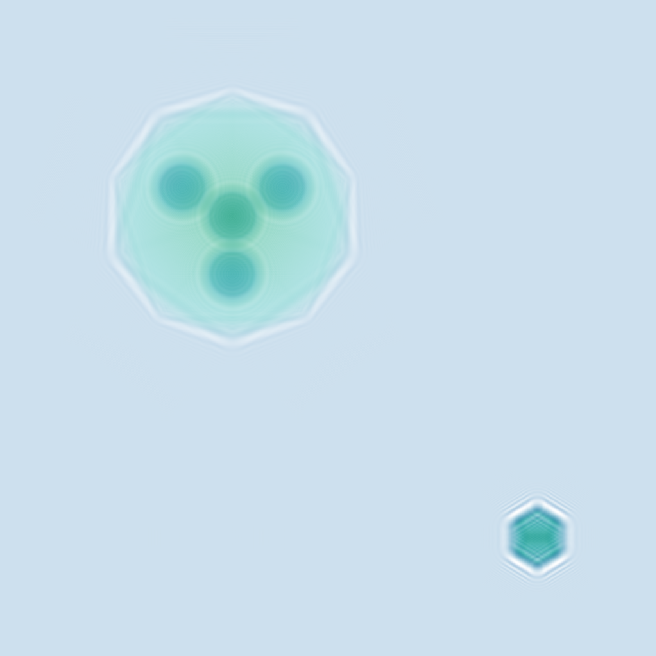
\includegraphics[width=\textwidth]{images/fig_simholo_v2_exitwave.png}}
		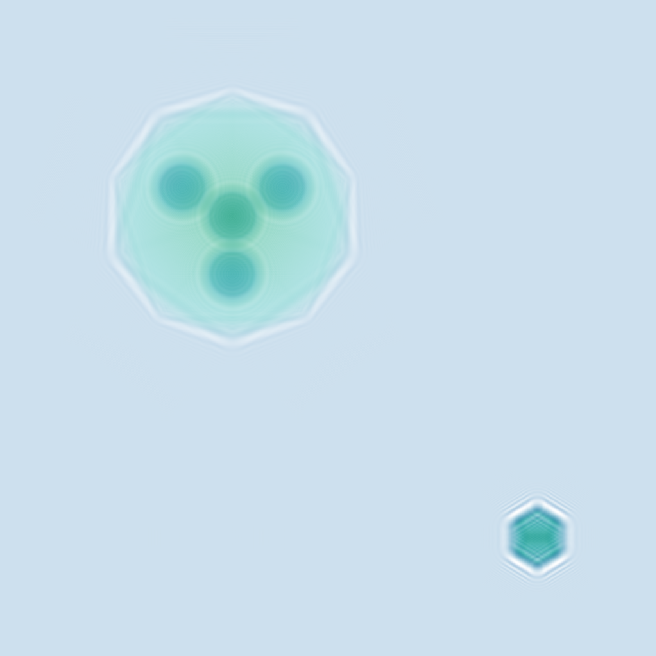
\includegraphics[width=\textwidth]{images/fig_simholo_v2_exitwave.png}\llap{\makebox[\wd1][l]{\includegraphics[width=0.4\textwidth]{images/fig_simholo_v2_exitwave_cw.pdf}}}
		\caption{Austrittswelle}
		\label{fig:komplexexit}
	\end{subfigure}	\hspace{2cm}
	\begin{subfigure}[b]{0.4\textwidth}
		\setbox1=\hbox{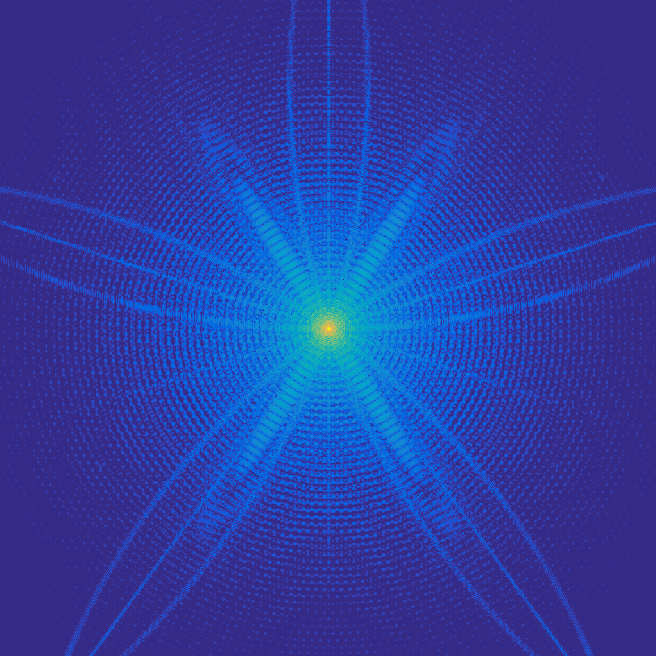
\includegraphics[width=\textwidth]{images/fig_simholo_v2_scatter.png}}
		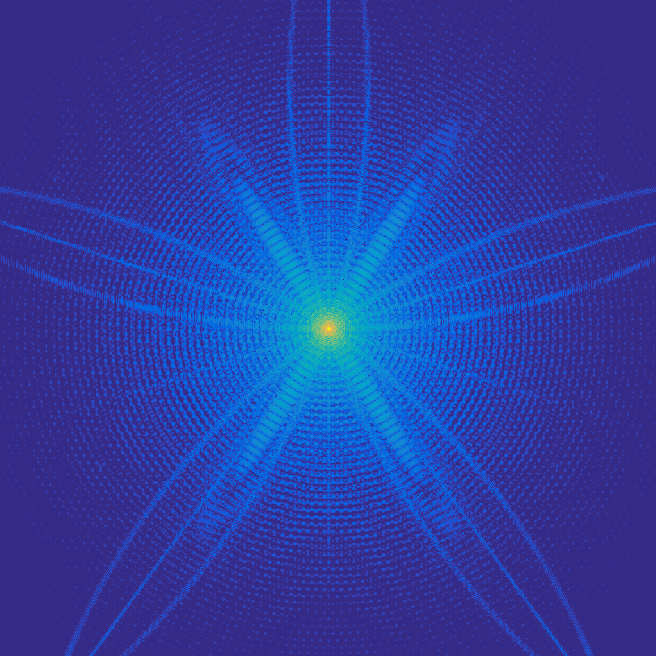
\includegraphics[width=\textwidth]{images/fig_simholo_v2_scatter.png}\llap{\makebox[\wd1][l]{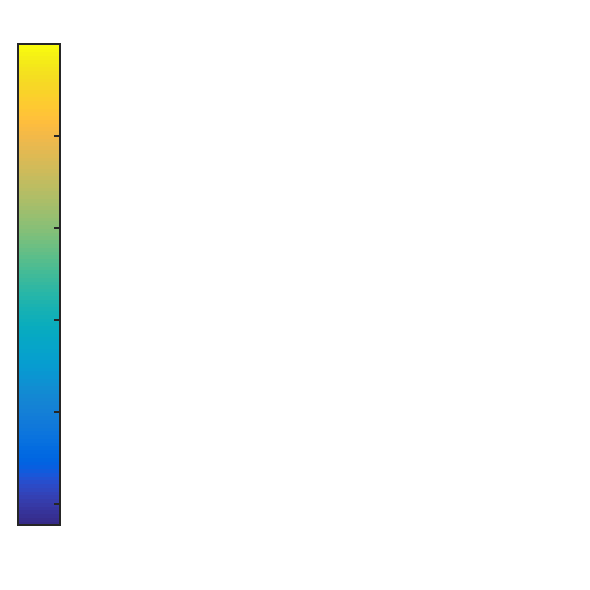
\includegraphics[width=0.5\textwidth]{images/fig_simholo_v2_scatter_cb.pdf}}}
			\caption{Streubild}
			\label{fig:komplexscatter}
	\end{subfigure}		
	\caption[Austrittswelle und Streubild eines komplexen Objektes]{Austrittswelle und logarithmiertes Streubild eines komplexen Objektes. Bei der Austrittswelle ist die relative Intensität bezüglich der Eintrittswelle über die Helligkeit dargestellt, die Phase über den Farbton.}
	\label{fig:komplex}
\end{figure}

\chapter{Rekonstruktion}
Nach XX entspricht die im Fernfeld aufgenommene Welle der Fouriertransformierten der Austrittswelle. Könnte sowohl Amplitude als auch Phase aufgenommen werden, so ließe sich durch eine einfache Rücktransformation die Austrittswelle rekonstruieren und somit Informationen über das Objekt gewinnen. Jedoch wird mittels eines Sensors nur die Intensität der Welle aufgezeichnet, die Informationen über die Phase gehen somit verloren. Das Problem, aus dieser unvollständigen Messung die Austrittswelle zu rekonstruieren wird als das Phasenproblem bezeichnet. Zur Lösung existiert u.A. der Ansatz der Freiflug-Holographie sowie die Methode der iterativen Phasenrekonstruktion
\section{Holographie}
Angenommen neben dem Objekt, über das Informationen gewonnen werden sollen befindet sich ein weiteres (im Weiteren als Referenz bezeichnetes) Objekt im Strahl, sodass die eingehende Welle an beiden gestreut wird. Sind Objekt und Referenz Näherungsweise 2D-Objekte in einer gemeinsamen Ebene, so gilt für die Austrittswelle $\phi_1$
\begin{equation}
	\phi_1=O+R
\end{equation}
mit $O$,$R$ den Austrittswellen von Objekt und Referenz. Für die aufgenommene Intensität $I$ im Fernfeld gilt
\begin{equation}
I=\left|\mathscr{F}\left[O\right]+\mathscr{F}\left[R\right]\right|^2=\left|\tilde{O}+\tilde{R}\right|^2
\end{equation}
Wird nun auf $I$ eine inverse Fouriertransformation angewendet,

\begin{equation}
	\mathscr{F}^{-1}\left[\left|\tilde{O}+\tilde{R}\right|^2\right]=
	\mathscr{F}^{-1}\left[\tilde{O}\tilde{O}^*\right]+
	\mathscr{F}^{-1}\left[\tilde{R}\tilde{R}^*\right]+
	\mathscr{F}^{-1}\left[\tilde{R}\tilde{O}^*\right]+
		\mathscr{F}^{-1}\left[\tilde{O}\tilde{R}^*\right]
\end{equation}
so ergibt sich mit Hilfe der komplexen Konjugation der Fouriertransformation XX und des Korrelationstheorems XX
\begin{equation}
\mathscr{F}^{-1}[I]\propto \underbrace{O \otimes O + R\otimes R}_{\text{Autokorrelationen}}+\underbrace{R\otimes O+ O\otimes R}_{\text {Kreuzkorrelationen}}
\end{equation}
Die Autokorrelationen, d.h. die Korrelation von Objekt und Objekt bzw Referenz mit Referenz liegen hierbei um den Ursprung des Koordinatensystems und können in jede Richtung maximal die doppelte Größe von Objekt bzw Referenz haben. Die Kreuzkorrelationen aus Objekt und Referenz sind punktsymmetrisch zum Ursprung und haben von diesem den gleichen Abstand wie Objekt- und Referenzaustrittswelle voneinander.
Sie  entsprechen einer Faltung des Objektes mit der gespiegelten, komplex konjugierten Referenz bzw der Referenz mit einem gespiegelten, komplex konjugierten Objekt.  Ist die Referenz in guter Näherung punktförmig und lässt sich durch eine Delta-Funktion beschreiben, so ist die Kreuzkorrelation näherungsweise die Austrittswelle des Objektes. Somit können trotz der verlorenen Phaseninformationen die Austrittswelle des Objektes inklusiver der Phase wieder gewonnen werden. Dieses Verfahren wird als im weiteren als Fouriertransformations-Holografie (FTH) bezeichnet.
\subsection{Entfaltung}
Um bei ausgedehnten Referenzen eine bessere Approximation des Objektes zu erhalten, muss die Faltung zwischen Objekt und Referenz rückgängig gemacht werden. Nach  XXX entspricht die Faltung einer Multiplikation, die Inverse somit einer Division im Fourierraum. Jedoch verursachen sowohl Rauschen wie auch Singulariäten in der fouriertransformierten Referenz Probleme.

Das Problem der Entfaltung tritt in verschiedenen Bereichen auf, unter anderem in der Bildverarbeitung.
Hier ist der Prozess der Wiener Entfaltung etabliert. 

Für Rauschen, dass nicht mit dem Signal korreliert ist stellt dies die Lösung...

\section{iterative Phasenrückgewinnung}
Wäre neben der Amplitude auch Phase der Fouriertransformation der Austrittswelle bekannt, so könnte diese durch eine inverse Transformation wiederhergestellt werden. 
Da bei N komplexen Datenpunkten im Realraum die Fouriertransformation durch N Amplituden und N Phasen, also 2N Variablen dargestellt werden kann, jedoch nur N Variablen (die Fourieramplituden) gemessen werden können, ist das Problem unterbestimmt und nicht eindeutig lösbar. Kann jedoch das zu rekonstruierende Objekt im Realraum auf N/2 Bildpunkte beschränkt werden, so wird das Problem lösbar. Die räumliche Beschränkung im Realraum wird 
durch die Wahl eines sog. Supports, außerhalb dessen der Realraum als leer angenommen wird umgesetzt.  
Die Problemstellung ist nun eine Lösung der Gleichung $\rho(x)=\mathscr{F}^{-1}\tilde{\rho}(q)$ unter den Nebenbedingungen dass 1. $\rho$ auf den Support beschränkt ist und 2. die Amplituden von $\tilde{\rho}$ mit den bekannten Fourieramplituden $A(q)$ übereinstimmt. 
\subsection{Algorithmen}
Ein zur Lösung der Problemstellung verwendeter Algorithmus, der Error-Reduction Algorithmus (ER) basiert auf abwechselnden Erzwingen der der Nebenbedingungen, d.h. von einem Startwert $\rho_0$ ausgehend wird zunächst $\tilde{\rho_0}$ bestimmt, die Amplitude im Fourierraum durch $A$ ersetzt, in den Realraum transformiert und dort außerhalb des Supports gleich Null gesetzt. Dies wird iterativ wiederholt, wobei sich $\rho_n$ einer beide Nebenbedingungen erfüllenden Lösung annähert.

Das Erzwingen der Nebenbedinung im Realraum kann als Projektion auf die Lösungsmenge $S$ der Nebenbedingung  mit dem Komplement $\bar{S}$ durch den Projektor $P_s$ 

 \begin{align}
 P_s\rho (x)=\begin{cases}
 \rho (x)  &\text{für } x\in S\\
 \mathbb{0}  &\text{für }x\notin S
 \end{cases}&&
 P_{\bar{s}}\rho (x)=\begin{cases}
 \mathbb{0} &\text{für } x\in S\\
 \rho (x)   &\text{für }x\notin S
 \end{cases}
 \end{align}
aufgefasst werden. Der analoge Projektor für die Erfüllung der Nebenbedingung im Fourierraum, der im Fourierraum die Amplitude von $\tilde{\rho}$ durch die bekannte Amplitude $A(q)$ ersetzt und dabei den Winkel $\Phi(q)$ beibehält lautet
\begin{align}
	\tilde{P}_m \bar{\rho}(q)&=A(q)e^{i\Phi(q)} &&P_m\rho(q)=\mathscr{F}^{-1}A(q)e^{i\Phi(q)}\mathscr{F}\rho(x)
\end{align}

	\begin{figure}
		\centering
		
\includegraphics[width=0.75\textwidth]{images/projektor.eps}
		\caption[Abbildungstext im Abbildungsverzeichnis]{Verwendete Projektoren. Der Support Projektor $P_S$ projiziert auf die durch den Support beschriebene Mannigfaltigkeit, $P_{\bar{S}}$ auf das Komplement. Ein Reflektor wendet die doppelte Schrittweite wie ein Projektor an und stellt somit eine Spiegelung an der Lösungsmenge der Nebenbedingung dar. Der Fourier-Projektor stellt in Fourierraum eine projektion auf die Kreisförmige Menge der bekannten Amplituden dar.}
		\label{fig:projektoren}
	\end{figure}.
	Neben den Projektoren die, den Schritt $\rho\rightarrow (\mathbb{1}+(P-\mathbb{1}))\rho$ ausführen, können auch sogenannte Reflektoren mit doppelter Schrittweite
	\begin{equation}
	R_\nu= (\mathbb{1}+2(P-\mathbb{1}))=(2P_\nu-\mathbb{1})
	\end{equation}
	eingeführt werden.
In dieser Schreibweise können auch Weiterentwicklungen wie der Hybrid Input Output (HIO) und Relaxed Averaged Alternating Reflections (RAAR) Algorithmus dargestellt werden XXTabelleXX. Ihre Prinzip ist in XXX graphisch dargestellt.
	\begin{figure}
		\centering
		
\includegraphics[width=0.75\textwidth]{images/algorithmen.eps}
		\caption[Abbildungstext im Abbildungsverzeichnis]{Darstellung der Algorithmen ER, RAAR und HIO. Bei ER findet eine abwechselnde Projektion auf die Lösungsmengen der Nebenbedinungen statt. Bei ER und HIO ist der einzelne Iterationsschritt komplexer und abhängig von einem Parameter $\beta$. Abbildung für ER und HIO nach \cite{XX}}
		\label{Abb:BspAbbildung}
	\end{figure} 
\subsection{Support}
Üblicherweise ist der Bereich auf den das Objekt im Realraum beschränkt ist nicht bekannt, der für die iterativen Rekonstruktionsalgorithmen benötigten Supports muss zunächst bestimmt werden. Hierfür existieren verschiedene Möglichkeiten. Die triviale Methode besteht aus einer Festlegung aus zuvor bekannten Dimensionen des Experiments. Jedoch kann nur in Ausnahmefällen so der Support ausreichend eng gewählt werden um die Bedingung XXX zur erfüllen.
Eine verbreitete Methode, bezeichnet als Shrink-Wrap Algorithmus, ist durch eine Anpassung des Supports während der Rekonstruktion gekennzeichnet: Der zunächst geratene (für eine eindeutige Lösung des Problems  zu große) Support wird nach einer festgelegten Anzahl an Rekonstruktionsiterationen auf den Bereich beschränkt, in dem die Rekonstruierte Intensität höher als ein festgelegter Schwellwert ist. Dieser aktualisierte Support wird für weitere Iterationen genutzt und erneut aktualisiert\cite{marchesini2003}.
Die aus der Holographie gewonnene Rekonstruktion des Objektes und eine Schätzung der Referenz lassen sich zu einem Support kombinieren. Der nötige Abstandsvektor dieser Supportteile ist der  Abstandsvektor zwischen Auto- und Kreuzkorrelation (XXX).

Abbildung
	\begin{figure}
		\centering
		
\includegraphics[width=0.75\textwidth]{images/support.eps}
		\caption[Abbildungstext im Abbildungsverzeichnis]{Erzeugung des Supports. Oben: Bei verwendung von Freiflug Holographie kann die Kreuzkorrelation aus Referenz und Objekt als Support genutzt werden. Zusätzlich muss im gleichen Abstand wie Kreuz und Autokorrelation die Referenz dem Support hinzugefügt werden. Unten: Der Shrinkwrap Alorithmus beginnt mit der Autokorrelation als initalem Support und passt diesen im laufe der Rekonstruktion an.}
		\label{Abb:BspAbbildung}
	\end{figure} 
\section{Vergleich}	
Somit können drei unterschiedliche Arten der Rekonstruktion betrachtet werden
\begin{itemize}
\item FTH mit Entfaltung
\item IPR mit Shrinkwrap-Support
\item IPR mit FTH Support
\end{itemize}

Die Rekonstruktionsansätze werden bezüglich Ihrer Empfindlichkeit für Rauschen, Hochpass und Fehler in der Abschätzung der Referenz untersucht. Dies geschieht zunächst mit rein synthetischen 2D Bildern als Ersatz für Austrittswellen um die Funktion der drei Ansätze und ihre Limitationen zu überprüfen.

\subsection{Einfluss Rauschen}
Zur Beurteilung des Einflusses von Rauschen auf die Rekonstruktionen werden die Fourieramplituden mit verschiedenen Auflösungen diskretisiert und ein Poisson-Rauschen angewendet.
\subsection{Einfluss Hochpass}
Der Einfluss des in Experimenten durch die nötige Blockierung des zentralen Strahles bedingten Hochpasses
\subsection{Einfluss Referenzabschätzung}
Sowohl für die Entfaltung wie auch für die festlegung des Supports für die iterative Rekonstruktion muss die Referenz abgeschätzt werden. Der Einfluss der Güte dieser Abschätzung..

\section{3D Austrittswelle}
Die für 2D-Bilder getesteten Ansätze können nun zur Rekonstruktion der Austrittswelle hinter einem 3D-Objekt eingesetzt werden. Die Dreidimensionalität des Objektes wird an dieser Stelle ignoriert und die Austrittswelle analog zu den 2D-Bildern betrachtet.
\section{Ausblick}

\chapter{Ausblick}
Die 3d-Eigenschaften des Objektes bislang bei der Rekonstruktion ignoriert

Refokussierung der Austrittswelle auf direkt hinter dem Objekt möglich

Das bestehende Framework aus Simulation, Mie-Validierung und Rekonstruktion ließe sich nun nuntzen um die 3d-Rekonstruktionen genauer zu untersuchen


%%%%%%%%%%%%%%%%   ANHANG   %%%%%%%%%%%%%%%%%%
\begin{appendices}
	\chapter{Detaillierte Abbildungen}
\section{Simulation}
Hier für verschiedene Parameter das gleiche radial provil bild wie im hauptteil

\section{Rekonstruktion}
	\chapter{Fourier Transformation}
Die in dieser Arbeit verwendete Form der Fouriertransformation lautet
\begin{equation}
	\mathscr{F} [f(\vec{x})] (\vec{q})
	=
	\frac{1}{(2\pi)^{\sfrac{n}{2}}}
	\int_{-\infty}^{\infty}
	f(\vec{x})
	e^{-i\vec{q} \cdot \vec{x} } 
	\dif  \vec{x}
\end{equation}
mit der inversen Fouriertransformation
\begin{equation}
	\mathscr{F}^{-1} [\tilde{f}(\vec{q})] (\vec{x})
	=
	\frac{1}{(2\pi)^{\sfrac{n}{2}}}
	\int_{-\infty}^{\infty}
	\tilde{f}(\vec{q})
	e^{i\vec{q} \cdot \vec{x} } 
	\dif  \vec{q} \, .
\end{equation}
Für diese gilt unter anderem: 
\paragraph{komplexe Konjugation}
\begin{align}
	\label{eq:ft_konjugation}
\mathscr{F}^{-1}\left[ \left(\mathscr{F}\left[f(x)\right]\right)^*  \right]	=f(-x)
\end{align}
$\rightarrow$ eine komplexe Konjugation im Fourierraum entspricht einer Spiegelung im Realraum
\paragraph{doppelte Fouriertransformation}
\begin{align}
	\mathscr{F}\left[\mathscr{F}\left[f(x)\right]  \right]	=f(-x)
\end{align}
$\rightarrow$ die zweimalige Anwendung der Fouriertransformation entspricht einer Spiegelung
\paragraph{Faltungstheorem}
\begin{align*}
	\label{eq:ft_faltung}
	\mathscr{F} [f\ast g] & =(2\pi)^{\sfrac{n}{2}}\mathscr{F}[f] \mathscr{F}[g]     \\
	\mathscr{F}[fg]       & =\frac{1}{(2\pi)^{\sfrac{n}{2}}}\mathscr{F}[f]\ast \mathscr{F}[g] \numberthis
\end{align*}
$\rightarrow$ eine Faltung im Realraum entspricht einer Multiplikation im Fourierraum
\paragraph{Korrelationstheorem}
\begin{align}
	\label{eq:ft_korrelation}
	\mathscr{F} [f\otimes g] & =(2\pi)^{\sfrac{n}{2}}\mathscr{F}[f] (\mathscr{F}[g])^*     \\
\end{align}
$\rightarrow$ eine Korrelation mit einer Funktion im Realraum entspricht im Fourierraum einer Multiplikation mit der komplex-konjugierten Funktion

\paragraph{Ableitung}
\begin{align}
\label{eq:ft_ableitung}
	\mathscr{F} [\pd{f(x)}{x}] (q)=-iq	\mathscr{F} [f] (q)   \\
\end{align}
$\rightarrow$ eine Ableitung  im Realraum wird zu einer Multiplikation im Fourierraum.

	\chapter{Mie-Streuung}
\label{app:mie}
Für die Intensität bei einem Streuwinkel $\theta$ gilt in der Mie-Theorie für die Streuung unpolarisierter Strahlung in Abhängigkeit von der Brechzahl $\eta$ der Sphäre (Radius $r$) und dem Parameter $x=r/k$:
\begin{equation}
	I(\theta)\propto\frac{1}{2}\left(\abs{S_1}^2+\abs{S_2}^2\right)
\end{equation} 
mit den Reihen
\begin{align}
	S_1=\sum_n{\frac{2n+1}{n(n+1)}(a_n\pi_n+b_n\tau_n)} &   & S_2=\sum_n{\frac{2n+1}{n(n+1)}(a_n\tau_n+b_n\pi_n)}\,, 
\end{align}
wobei die Reihen bei der numerischen Auswertung nach $N$ Termen abgebrochen werden. Eine hinreichende Konvergenz liegt meist bei $N\approx2+x+4\sqrt[3]{x}$ Termen vor.  $\pi_n$ und $\tau_n$ können mit $\pi_1=1$ und  $\pi_2=3\cos{\theta}$ rekursiv über die Relationen
\begin{align}
	  & \pi_n=\frac{2n-1}{n-1}\cos{\theta}\pi_{n-1}-\frac{n}{n-1}\pi_{n-2} &   & \tau_n=n\cos{\theta}\pi_n-(n+1)\pi_{n-1}
\end{align}
und $a_n$,$b_n$ über 
\begin{align}
	a_n=\frac{(D_n/\eta+n/x)\psi_n-\psi_{n-1}}{(D_n/\eta+n/x)\chi_n-\chi_{n-1}} &   &   
	b_n=\frac{(\eta D_n+n/x)\psi_n-\psi_{n-1}}{(\eta D_n+n/x)\chi_n-\chi_{n-1}}
\end{align} definiert werden. $D_n$ lässt sich rekursiv über
\begin{align}
	D_{n-1}=\frac{n}{\eta*x}-\frac{1}{D_n+n/(\eta x)} 
\end{align} 
berechnen. Dabei kann ausgenutzt werden, dass bei dieser Berechnung der Fehler strikt monoton fallend ist, d.h. wird $D_{N'}$ für ein hinreichend großes $N'>N$ abgeschätzt, so ist der Fehler von $D_n$ für $n<N$ hinreichend genau. Hierbei hat sich $N'=N+15$ und die Abschätzung $D_{N'}=0$ bewährt. Mittels sphärischer Besselfunktionen 1. Art ($j_n$) und 2. Art ($y_n$) können $\psi_n$ und $\chi_n$ mittels
\begin{align}
	\psi_n=x j_n &   & \chi_n=x j_n+ixy_n 
\end{align}
berechnet werden~\cite{bohren1983,maetzler2002}.


	\chapter{Algorithmen zur Phasenrückgewinnung}
\label{chap:anhang_algos}
Die grundlegende Iteration der iterativen Rekonstruktionsalgorithmen ER, HIO und RAAR in ihrer Projektionsschreibweise sind in \Fref{tab:ipr} dargestellt \cite{fienup1978,luke2004,marchesini2007}.

Aus Gründen der Simplizität wird davon ausgegangen, dass die Realraumbeschränkungen nur den Support beinhalten, d.h. der Realraum-Projektor $P_s$ geschrieben werden kann als 
\begin{align}
	P_s\rho (x)=\begin{cases}
	\rho (x)  &\text{für } x\in S\\
	\mathbb{0}  &\text{für }x\notin S
	\end{cases} &   &   
	P_{\bar{s}}\rho (x)=\begin{cases}
	\mathbb{0} &\text{für } x\in S\\
	\rho (x)   &\text{für }x\notin S
	\end{cases}
\end{align}
und somit als reiner Support-Projektor aufgefasst werden kann. In der Literatur wird unter der Bezeichnung $P_s$ teilweise auch ein Projektor bezeichnet der außerdem weitere Forderungen im Realraum beinhaltet. Im Rahmen dieser Arbeit nur für den ER-Algorithmus zusätzlich eine Form implementiert, deren Realraum-Projektor eine reele, positive Lösung erzwingt (\texttt{reconstruction/ERiterRealPos.m}), da das mittelfristige Ziel die Rekonstruktion der Austrittswelle inklusive der relativen Phasenbeziehungen darstellt.
 
Für den HIO-Algorithmus gilt mit jenem $P_s$ 
\begin{align*}
	\begin{rcases}	
	P_m\rho_n                               & \text{für } x\in S    \\
	\left[\mathbb{1}-\beta P_m\right]\rho_n & \text{für } x\notin S 
	\end{rcases}	
	=\left[P_sP_m+\left(P_{\bar{s}}-\beta P_{\bar{s}} P_m\right)\right]\rho_n
	\,.
\end{align*}
Diese Form erleichtert das Verständnis von \fref{fig:recon}. Zum weiteren Verständnis ist in \fref{fig:raar} der Prozess für den RAAR-Algorithmus schrittweise dargestellt.
	
Die implementierte Form des RAAR Algorithmus' basiert auf folgender Umformung:
\begin{align*}
	\frac{\beta}{2}\left(R_sR_m+\mathbb{1}\right)
	                              & =\frac{\beta}{2}\left((2P_s-\mathbb{1})(2P_m-\mathbb{1})+\mathbb{1}\right) 
	=2\beta P_sP_m-\beta P_s-\beta P_m+\beta\mathbb{1}\\
	\frac{\beta}{2}\left(R_sR_m+\mathbb{1}\right)+\left(1-\beta\right) P_m
	                              & =2\beta P_sP_m+\beta (\mathbb{1}-P_s)+ (1-2\beta)P_m                       \\
	                              & =                                                                          
	\begin{cases}
	P_m                           & \text{für } r\in S                                                        \\
	(1-2\beta)P_m+\beta\mathbb{1} & \text{für } r\notin S                                                     
	\end{cases}\\
\end{align*}
\begin{table}
	\centering
	\begin{tabular}{cc}
		\hline\hline
		Algorithmus                             & $\rho_{n+1}$                                                                               \\ 							
		\hline
		ER                                      & $P_sP_m\rho_n$                                                                             \\ 								
		HIO                                     & $\begin{cases}                                                                             
		P_m\rho_n                               & \text{für } x\in S                                                                        \\
		\left[\mathbb{1}-\beta P_m\right]\rho_n & \text{für } x\notin S                                                                     
		\end{cases}$\\
		RAAR                                    & $\left[\frac{\beta}{2}\left(R_sR_m+\mathbb{1}\right)+\left(1-\beta\right)P_m\right]\rho_n$ \\																
		\hline\hline
	\end{tabular}
	\caption[IPR-Algorithmen]{Iterationsschritte der implementierten IPR-Algorithmen.}
	\label{tab:ipr}
\end{table}	

\begin{figure}
	\centering
	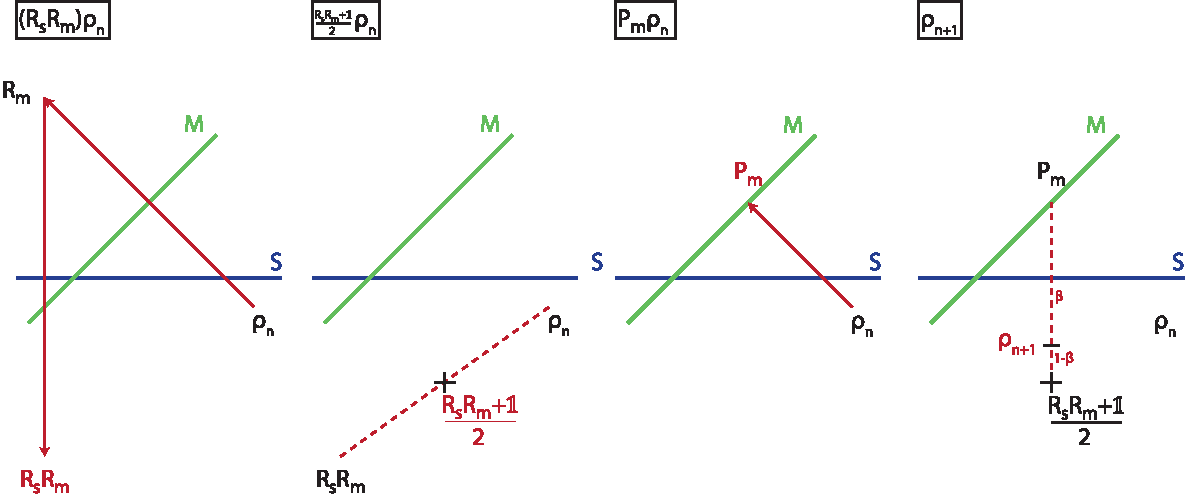
\includegraphics[width=1\textwidth]{images/raar.pdf}
	\caption[RAAR]{Detailierte Darstellung von \fref{fig:recon} für RAAR, von links nach rechts: 1. Die Anwendung des Modulus-Reflektors gefolgt vom Support-Reflektor liefert $R_sR_m\rho$. 2. Der Mittelpunkt von $R_sR_m\rho$ und $\rho$ ist $(\sfrac{1}{2}R_sR_m+\mathbb{1})\rho$. 3. Anwenden des Modulus-Projektors liefert $P_m\rho$. 4. Die Kombination von $P_m\rho$ und $(\sfrac{1}{2}R_sR_m+\mathbb{1})\rho$ im Verhältnis $\beta$ und $1-\beta$ liefert das Ergebnis der Iteration  und somit den Startpunkt für die nächste Iteration ($\rho_{n+1}$).}
	\label{fig:raar}
\end{figure} 	

	\chapter{Programmüberblick}
Überblick über die erstellten Matlab-Funktionen. Der vollständige Programmcode ist unter XXX abrufbar.
 
%\subsection*{Hilfsfunktionen}
%\begin{description}[style=nextline]
%	\item [\textit{[data]=\textsc{ft2}(data)}]
%		GPU-optimierte Version von fftshift(fft2(fftshift(data))) für grade N
%	\item [\textit{[data]=\textsc{ift2}(data)}]
%		GPU-optimierte Version von fftshift(ifft2(fftshift(data))) für grade N
%\end{description}
\subsection*{Erzeugung von Objekten}
\subsection*{Simulation}
\begin{description}[style=nextline]
	\item [\textit{[theta,Intensity,S1,S2]=\textsc{mie}(lambda,radius,beta,delta,steps)}]
		Intensität in Mie Streuung unpolarizierten Lichtes an Sphäre mit Radius 'radius' (in nm)
		und Brechzahl n=1-delta+ibeta bei Wellenlänge lambda (in nm), ausgewertet in
		'steps' linearen Schritten des Winkels theta)
\end{description}
\begin{description}[style=nextline]
	\item [\textit{[out]=\textsc{msft}(wavelength,objects,N,dx,gpu)}]
\end{description}
\begin{description}[style=nextline]
	\item [\textit{[out]=\textsc{multislice}(wavelength,objects,N,dx,gpu)}]
\end{description}
\begin{description}[style=nextline]
	\item [\textit{[out]=\textsc{thibault}(wavelength,objects,N,dx,gpu)}]
\end{description}



\subsection*{Rekonstruktion}
\begin{comment}


Hilfmittel
	ft2
	ift2
	maskfilter
	pad2size
Simulation
	Erzeugun von Objekten
		
	-msft
	-multislice
	-thibault

Rekonstruktion
	-wiener
	-reconstruct
	SW
	holo\_support
	ERiter
	RAARiter
	HIOiter
	\end{comment}
\end{appendices}



%%%%%%%%   ABBILDUNGSVERZEICHNIS   %%%%%%%%%%%

\listoffigures
\addcontentsline{toc}{chapter}{Abbildungsverzeichnis}
\cleardoublepage


%%%%%%%%%   TABELLENVERZEICHNIS   %%%%%%%%%%%%

\listoftables
\addcontentsline{toc}{chapter}{Tabellenverzeichnis}
\cleardoublepage


%%%%%%%%%   LITERATURVERZEICHNIS   %%%%%%%%%%%

\bibliography{ffz}
\bibliographystyle{unsrt}
\addcontentsline{toc}{chapter}{Literaturverzeichnis}
\cleardoublepage




\end{document}